% SCD07.tex         latex SCD07; bibtex SCD07; dvips SCD07; ps2pdf SCD07
% $Author: predrag $ $Date: 2019-05-13 15:05:44 -0400 (Mon, 13 May 2019) $

% Predrag renamed to SCD07.tex from rpo.tex     2019-05-12
% Predrag resubmission edits                    2009-04-07


\input type

\ifdraft
    % this style while editing: double spaced, draft
    % \documentclass[draft]{siamltex}     % without figs
    \documentclass{siamltex}          % with figs

\else
    % double spaced, for submission
    % \documentclass[pre,preprint,groupedaddress,showpacs,showkeys]{revtex4}
    % this style for arXiv version, in the journal layout:
    \documentclass[final]{siamltex}
\fi



\input defs     % all definitions in defs.tex


                \begin{document}
                \title{
\edit{On s}tate space geometry of the
Kuramoto-Sivashinsky flow \edit{in a periodic domain}
                 }
                  \author{
Predrag Cvitanovi\'c\footnotemark[1],
Ruslan L. Davidchack\footnotemark[2],
    and
Evangelos Siminos\footnotemark[1]
                    }

                \maketitle

\renewcommand{\thefootnote}{\fnsymbol{footnote}}
\footnotetext[1]{
          School of Physics,
          Georgia Institute of Technology, Atlanta, GA 30332-0430, USA
                          }
\footnotetext[2]{
Department of Mathematics, University of Leicester,
            University Road, Leicester LE1 7RH, UK
                }
\renewcommand{\thefootnote}{\arabic{footnote}}

                \begin{abstract}
The continuous and discrete symmetries of the
Kuramoto-Sivashinsky system restricted to a spatially
periodic domain play a prominent role in shaping the
invariant sets of its chaotic dynamics. The continuous
spatial translation symmetry leads to relative
\edit{equilibrium} (traveling wave) and relative periodic
orbit \edit{(modulated traveling wave)} solutions. The
discrete symmetries lead to existence of {equilibrium} and
periodic orbit solutions, induce decomposition of state space
into invariant subspaces, and enforce certain structurally
stable heteroclinic connections between equilibria. We show,
on the example of a particular small-cell Kuramoto-Sivashinsky
system, how the geometry of its dynamical state space is
organized by a rigid `cage' built by heteroclinic connections
between equilibria, and demonstrate the preponderance of
unstable relative periodic orbits and their likely role as
the skeleton underpinning spatiotemporal turbulence in
systems with continuous symmetries. We also offer novel
visualizations of the high-dimensional Kuramoto-Sivashinsky
state space flow through projections onto low-dimensional,
PDE representation independent, dynamically invariant
intrinsic coordinate frames, as well as in terms of the
physical, symmetry invariant energy transfer rates.
                \end{abstract}

\begin{keywords}
relative periodic orbits, chaos, turbulence, continuous symmetry, {\KSe}
\end{keywords}

\begin{AMS}
35B05, 35B10, 37L05, 37L20, 76F20, 65H10, 90C53
\end{AMS}

\pagestyle{myheadings}
\thispagestyle{plain}
\markboth{P.~CVITANOVI\'C, R.~L. DAVIDCHACK, AND E.~SIMINOS}
         {GEOMETRY OF \edit{THE} KURAMOTO-SIVASHINSKY FLOW}

\ifsvnmulti
 \svnkwsave{$RepoFile: lyapunov/intro.tex $}
 \svnidlong {$HeadURL: svn://zero.physics.gatech.edu/siminos/lyapunov/intro.tex $}
 {$LastChangedDate: 2016-03-06 15:29:29 -0500 (Sun, 06 Mar 2016) $}
 {$LastChangedRevision: 4688 $} {$LastChangedBy: predrag $}
 \svnid{$Id: intro.tex 4688 2016-03-06 20:29:29Z predrag $}
\fi

\chapter{The physical dimension of a \KS\ flow}
    \label{c-draft}

Bits and pieces for a putative article.

\section{Introduction}
\label{sect:intro}

Inspired by the global
studies of \refrefs{PoGiYaMa06,ginelli-2007-99,YaTaGiChRa08,TaGiCh09} of
`{\cLvs}' we use Floquet vectors of unstable \po s to
identify the \emph{local} number of degrees of freedom that capture the
physics of a `turbulent' PDE on a compact spatial domain. That number is
proportional to the system size, for \KS\ flow roughly four times the
number of positive/marginal Floquet (or Lyapunov) exponents, and twice its
Kaplan-Yorke estimate.

The idea is to coarsely cover the \emph{continuous-symmetry reduced}
nonlinear strange attractor with a set of hyperplanes\rf{SiCvi10,FrCv11},
as in \reffig{fig:Tesselate}. Any adjacent pair intersects in a `ridge'
hyperplane of one less dimension. So our task is to, for a given strange
attractor, pick a set of {\PoincSec}-fixing points, such that each local
section is approximately tangent to the strange attractor. For simplicity
here we shall consider only the flows with a 1 continuous parameter (the
time), postponing the more general case of continuous symmetries to a
happier time. An example of such dynamics is the \KS\ flow restricted to
the antisymmetric subspace\rf{Christiansen97,lanCvit07}; some examples of
flows with continuous symmetries are the \KS\ flow on a periodic
domain\rf{SCD07}, the pipe flow\rf{ACHKW11} and the \pCf\rf{GHCW07}.

We propose to construct a global atlas by deploying a finite
number of linear {\PoincSec s} in
neighborhoods of the most important equilibria and/or periodic orbits
as local charts.
This is the periodic-orbit implementation of the idea of {\statesp\
tessellation} so dear to professional cyclists, \reffig{fig:Tesselate}.

% In FrCv11.tex replace by Tesselate.png
%%%%%%%%%%%%%%%%%%%%%%%%%%%%%%%%%%%%%%%%%%%%%%%%%%
\SFIG{f_1_08_1}
{}{
Smooth dynamics  (left frame) tesselated by the skeleton of periodic
points, together with their linearized neighborhoods, (right frame).
Indicated are segments of two 1-cycles and a 2-cycle that alternates
between the neighborhoods of the two 1-cycles, shadowing first one of the
two 1-cycles, and then the other.
}{fig:Tesselate} %{Hyp} %{fig6} and {tr:fig6} in ChaosBook
%
%%%%%%%%%%%%%%%%%%%%%%%%%%%%%%%%%%%%%%%%%%%%%%%%%%
%


\section{Charting the \statesp}
	\label{sec:chart}
% extracted from siminos/froehlich/slice/FrCv11.tex   2011-02-20

Work on \KS\ suggests how to proceed: it was shown in
\refrefs{lanCvit07,SCD07} that for turbulent/chaotic systems a set of
{\PoincSec s} is needed to capture the dynamics. The choice of
sections should reflect the dynamically dominant patterns seen in the
solutions of nonlinear PDEs. We propose to construct a global atlas of
the dimensionally \reducedsp\ $\pSRed$ by deploying linear {\PoincSec s} $\PoincS{}^{(j)}$ across neighborhoods of the qualitatively most important
patterns $\slicep{}^{(j)}$.
We shall refer to these states as \emph{\template s}, each
represented in the \statesp\ $\pS$ of the system by
a \emph{\template\ point} $\slicep$. Together with the velocity
field at this point, a template defines a linear {\PoincSec},
an affine hyperplane $\sspRed \in \PoincS$,
\beq
    \vel(\slicep) \cdot (\sspRed - \slicep)= 0
\,,
\ee{locTransvVar1}
locally normal to the $\vel(\slicep)$ at the \template\ point $\slicep$.
(For a discussion of inner products, see
\refappe{def:innerProduct}.)
(For a motivation, see
\refappe{s-POs-flows} \emph{Newton method for flows}.)
Each {\PoincSec} $\PoincS{}^{(j)}$, provides a local chart
at $\slicep{}^{(j)}$ for a
neighborhood of an important, qualitatively distinct class of solutions
(2-rolls states, 3-rolls states, \etc); together they `Voronoi'
tessellate  the curved manifold in which the reduced strange attractor is
embedded by a finite set of hyperplane
tiles\rf{rowley_reconstruction_2000,RoSa00}.

The physical task is to, for a given dynamical flow, pick a set of
qualitatively distinct {\template s} whose {\PoincSec s} are locally tangent
to the strange attractor\ES{Do you mean locally transverse?}.
A {\PoincSec} is a
($d\!-\!1$)\dmn\ hyperplane. If we pick another {\template} point
$\slicep{}^{(2)}$, it comes along with its own {\PoincSec}. Any
neighboring pair of $(d\!-\!1)$\dmn\ {\PoincSec s} intersects in a `ridge'
(`boundary,' `edge'), a $(d\!-\!2)$\dmn\ hyperplane, easy to compute.
A global atlas so constructed should be sufficiently
fine-grained: each `chart' or `tile,' bounded by ridges to
neighboring {\PoincSec s}, should be sufficiently small.

Follow an ant as it traces out a trajectory
$\sspRed{}^{(1)}(\tau)$, confined to the {\PoincSec} $\PoincS{}^{(1)}$
The
moment $\braket{(\sspRed{}^{(1)}(\tau)-\slicep{}^{(2)})}{\vel{}{}^{(2)}}$ changes
sign, the ant has crossed the ridge and  continues its merry stroll within the
$\PoincS{}^{(2)}$ {\PoincSec}.

There is a rub, though - you need to know how to pick the
neighboring {\template s}. This is a reflection of the flaw inherent in use
of a {\PoincSec} hyperplane globally: a {\PoincSec} is derived from the Euclidean
notion of distance, but for nonlinear flows the distance has to be
measured curvilinearly, along unstable
manifolds\rf{Christiansen97,DasBuch}. We nevertheless have to stick with
tessellation by linearized tangent spaces, as curvilinear charts appear
computationally prohibitive. Perhaps a glance at
\reffig{fig:Tesselate} helps visualize the problem; imagine that the
tiles belong to the
{\PoincSec s} through {\template} points on these orbits. One could slide
{\template s} along their trajectories until the pairs of straight line
segments connecting neighboring {\template} points are minimized, but
that is not physical: one would like the dynamical trajectories to cross
ridges as continuously as possible. So how is one to orient
the {\template s} relative to each other? The choice of the first template fixes all {\em
relative phases} to the succeeding {\template s}, as was demonstrated in
\refref{SCD07}: the universe of all other solutions is rigidly fixed
through a web of heteroclinic connections between them. This insight
garnered from study of a 1-dimensional \KS\ PDE is more remarkable still
when applied to the plane Couette flow\rf{GHCW07}, with 3-$d$ velocity
fields. The {\em relative phase} between
two {\template s} is thus fixed  by the shortest heteroclinic connection,
a rigid bridge from one neighborhood to the next. Once the relative phase
between the templates {\template s} is fixed, so are their their {\PoincSec s},
\ie, their tangent hyperplanes, and their intersection, \ie, the  ridge
joining them.

\section{Les r\`egles du jeu}
    \label{sec:defs}

% 2013-10-18 Predrag from \Chapter{stability}{13jun2013}{Local stability}

flow transports the
displacement $\deltaX (\zeit)$ along the trajectory
$\ssp(\xInit,\zeit) = \flow{\zeit}{\xInit}$
\beq
{d \over dt} \deltaX(\xInit,t) =
{\Mvar}(\ssp) \,  \deltaX(\xInit,t)
	\,,\qquad \ssp=\ssp(\xInit,t)
\, .
\label{lin_odes}
\eeq
\stabmat, %stability matrix
velocity gradients matrix (instantaneous rate of deformation)
\beq
{\Mvar}_{ij}(\ssp) ={\pde \vel_i(\ssp)\over \pde \ssp_j  }
\ee{DerMatrix}
The finite time $\zeit$
deformation of an infinitesimal neighborhood, with initial frame at $\xInit$,
into the co-moving, non-orthogonal frame at $\ssp(\zeit)$
is described by the eigen\-vectors and eigen\-values
\beq
\jMps^\zeit\, \jEigvec[k] = \ExpaEig_{k} \,\jEigvec[k]
\,,\qquad
j = 1,2, \cdots,d
\,.
\ee{cplxExpaEig1}
of the {\jacobianM} $\jMps^\zeit$
of the linearized flow
\beq
    \deltaX(t) = \jMps^\zeit(\xInit) \, \deltaX_0
    \,, \qquad
\jMps^\zeit_{ij}(\xInit)
  =  \frac{\pde \ssp(\zeit)_i}{\pde \ssp(0)_j}
    \,, \quad
\jMps^0(\xInit) = \matId
\, .
\label{hOdes}
\eeq
%
%\beq
% \jMps^t(\ssp_\stagn) = e^{{\Mvar}_\stagn t}
%    \,,\qquad
% {\Mvar}_\stagn={\Mvar}(\ssp_\stagn)
%\,.
%\ee{eqPointStab}
The symbol $\ExpaEig_k$ denotes the $k$th {\em eigen\-value}
({\em stability multiplier}) of the finite time {\jacobianM} $\jMps^\zeit$.
Symbol $\eigExp[k]$ will be reserved for the $k$th \emph{stability exponent},
with real part $\eigRe[k]$ and phase $\eigIm[k]$:
\beq
\ExpaEig_k = e^{\zeit \eigExp[k]}
    \,\qquad
\eigExp[k] = \eigRe[k] +i \eigIm[k]
\,.
\ee{stabExpon}
Stability multipliers are either real or
come in complex pairs,
\[
\{\ExpaEig_{k},\ExpaEig_{k+1}\}
= \{e^{\period{}(\eigRe[k] + i\eigIm[k])}, e^{\period{}(\eigRe[k] - i\eigIm[k])}\}
\,,
\]
with magnitude $|\ExpaEig_k|$ and phase $\eigIm[k]$.  The phase describes the
rotation velocity in the plane defined by the corresponding pair of
real orthogonal eigen\-vectors, $\{\Re\jEigvec[k],\Im\jEigvec[k]\}$,
with one period of rotation given by
\( %beq
    \period{} = 2\pi/\eigIm[k]
\,.
\) %ee{RotPeriod}
$\derf{t}{\xInit}$ depends on the initial point $\xInit$ and the
elapsed time $t$. For notational brevity we omitted this dependence,
but in general both the stability
multiplier and the eigenvectors,
\(
\ExpaEig_j = \ExpaEig_j(\xInit,t)
    \,,\; \cdots \,,\;
\jEigvec[j] = \jEigvec[j](\xInit,t)
\,,
\)
also depend on the trajectory traversed and the choice of
coordinates. We shall refer to the eigenvectors $\jEigvec[j]$ as
\emph{{\cLvs}}.

an important property of \jacobianMs\ is that they
are multiplicative along the flow,
\beq
\jMps^{\zeit+\zeit'}\!(\ssp)
    = \jMps^{\zeit'}\!(\ssp')\, \jMps^\zeit(\ssp), \qquad \mbox{where} \,\;
\ssp'=\flow{\zeit}{\xInit}
\,.
\ee{Jmultiplic}


Nearby trajectories separate along the {\em unstable directions},
approach each other along the {\em stable directions}, and change
their distance along the {\em marginal directions} at a rate slower
than exponential, corresponding to the eigen\-values of  the
{\jacobianM} with magnitude larger than, smaller than, or equal to 1.
One of the preferred directions is the
direction of the flow itself: $\jMps^{\zeit} (\xInit)$ transports
the velocity vector at $\xInit$ to the velocity vector at
$\ssp(\zeit)$:
\beq
\velField{\ssp(\zeit)} = \jMps^{\zeit} (\xInit) \,\velField{\xInit} \, .
\ee{JacobVeloc}

% 2013-10-18 Predrag from \Chapter{invariants}{17mar2013}{Cycle stability}
consider the case where $\ssp_\stagn$ is an \eqv\ point.
% \refeq{EquilPoint}.
The \stabmat\ ${\Mvar}={\Mvar}(\ssp_\stagn)$
is a constant matrix,
\( %beq
\flow{\zeit}{\ssp}
  = \ssp_\stagn + e^{{\Mvar} \zeit} (\ssp-\ssp_\stagn) + \cdots
\,,
\) %ee{EquilPtStab}
the {\jacobianM} of an \eqv\ point is
\beq
 \jMps^\zeit_\stagn = e^{{\Mvar_\stagn} \zeit}
    \,,\qquad
 \jMps^\zeit_\stagn =  \jMps^\zeit(\ssp_\stagn)
     \,,\;
 {\Mvar_\stagn}={\Mvar}(\ssp_\stagn)
\,.
\ee{eqPointStab}
The eigenvalues and the eigen\-vectors of \stabmat\  ${\Mvar}_\stagn$
\beq
{\Mvar}_\stagn \, \jEigvec[j]
   = \eigExp[j]_\stagn \,\jEigvec[j]
\,,
\ee{cplxEigExp}
describe the linearized neighborhood of the \eqv\ point, with
stability exponents
$\eigExp[j]_p = \eigRe[j]_p \pm i\eigIm[j]_p$
independent of any particular coordinate choice.
The eigenvectors are also the eigenvectors of the \jacobianM,
\( %beq
\jMps^\zeit_\stagn \, \jEigvec[j]
   = \exp({\zeit\eigExp[j]_\stagn })\,\jEigvec[j]
\,.
\) %ee{equilJacob}

$\jMps_{p}(\ssp) = \jMps^\period{}(\ssp)$ is the \jacobianM\
for a single traversal of the prime cycle $p$, $\ssp \in \pS_p$ is
any point on the cycle, and $f^{r\period{}}(\ssp)=\ssp$ as
$f^{t}(\ssp)$ returns to $\ssp$ every multiple of the period
$\period{}$.

The \jacobianM\ $\jMps_p(\ssp)$ depends upon $\ssp$ (the
`starting' point of the periodic orbit),
but its eigenvalues do not, so we
write the eigenvalue equation as
\beq
\jMps_{p}(\ssp)\, \jEigvec[j](\ssp)
   = \ExpaEig_{j} \,\jEigvec[j] (\ssp)
\,,
\ee{cplxExpaEig}
where $\ExpaEig_{j}$ are independent of $\ssp$, and we refer to
eigen\-vectors $\jEigvec[j]$ as `{\cLvs}', or, for \po s,
as `Floquet vectors'.

The time-dependent $\period{}$-periodic vector fields, such as the
flow linearized around a \po, are described by Floquet theory. Hence
from now on we shall refer to a \jacobianM\ evaluated on a periodic
orbit $p$ either as a [$d\!\times\!d$] {\em \FloquetM} $\jMps_p$ or a
 [$(d\!-\!1)\times(d\!-\!1)$] {\em \monodromyM} $\monodromy_p$, to its
eigenvalues $\ExpaEig_{j}$ as \emph{Floquet multipliers}
\refeq{cplxExpaEig}, and to $\eigExp[j]_p = \eigRe[j]_p+i\eigIm[j]_p$
as \emph{Floquet exponents}.
The stretching/contraction rates per unit time
are given by the real parts of {Floquet exponents}
\beq
\eigRe[j]_p = {1 \over \period{p}} \ln \left|\ExpaEig_{p,j}\right|
\,.
\ee{stabExps}
The factor ${1 / \period{p}}$ in the definition of the Floquet exponents
is motivated by its form for the linear dynamical systems.
A Floquet exponent is \emph{not} a Lyapunov
exponent evaluated on one period the prime cycle $p$.
When $\ExpaEig_{j}$ is real, we do care about
\(\sign{}^{(j)}
     =   \ExpaEig_{j}/|\ExpaEig_{j}|
     \in \{+1,-1\}
\,,
\)
the sign of the $j$th Floquet multiplier.
If $\sign{}^{(j)}  = -1$ and $|\ExpaEig_{j}| \neq 1$, the corresponding
eigen-direction is said to be {\em inverse hyperbolic}. Keeping track
of this by case-by-case enumeration is an unnecessary nuisance, so
most of our formulas will be stated in terms of the Floquet
multipliers $\ExpaEig_j$ rather than in the terms of the multiplier
signs $\sign{}^{(j)}$, exponents $\eigRe[j]$ and phases $ \eigIm[j]$.

The expanding directions, $|\ExpaEig_e| > 1$, have to be
taken care of first, while the contracting directions $|\ExpaEig_c| <
1$ tend to take care of themselves, hence one orders multipliers
$\ExpaEig_k$ in order of decreasing magnitude
\( %beq
| \ExpaEig_1 | \geq | \ExpaEig_2 |
    \geq \ldots \geq | \ExpaEig_d |
\,.
\) %ee{LambdaOrd}
Since $| \ExpaEig_j | = e^{t \eigRe[j]}$, this is the same as
ordering by
\( %beq
\eigRe[1] \geq \eigRe[2]
    \geq \ldots \geq \eigRe[d]
\,.
\) %ee{lambdaOrd}
We sort the {Floquet multipliers} $\{\ExpaEig_{p,1}$,
$\ExpaEig_{p,2}$, $\dots$, $\ExpaEig_{p,d}\}$ of the
\FloquetM\  evaluated on the $p$-cycle into three sets
$\{e,m,c\}$
\bea
\mbox{expanding:}
        &\quad \{ \ExpaEig \}_e &
        =\, \{ \ExpaEig_{p,j}: \left|\ExpaEig_{p,j}\right| > 1 \}
                \continue
        &\quad \{ \eigExp \}_e &
        =\, \{ \eigExp[j]_p:~\eigRe[j]_p > 0 \}
                \continue
\mbox{marginal:}
        &\quad \{ \ExpaEig \}_m &
        =\, \{ \ExpaEig_{p,j}: \left|\ExpaEig_{p,j}\right| = 1 \}
                \label{EigSorted}\\
        &\quad \{ \eigExp \}_m &
        =\, \{ \eigExp[j]_p:~\eigRe[j]_p = 0 \}
                \continue
\mbox{contracting:}
        &\quad \{ \ExpaEig \}_c &
        =\, \{ \ExpaEig_{p,j}: \left|\ExpaEig_{p,j}\right| < 1 \}
                \continue
        &\quad \{ \eigExp \}_c &
        =\, \{ \eigExp[j]_p:~\eigRe[j]_p < 0 \}
\,.
\nnu
\eea
The volume of expanding manifold plays an
important role. We denote by $\ExpaEig_{p}$ (no $j$th eigenvalue
index) the product of {\em expanding} Floquet multipliers
\beq
\ExpaEig_p=\prod_e \ExpaEig_{p,e}
\,.
\ee{expVol}

If {\em all} Floquet exponents (other than the vanishing longitudinal
exponent) of {\em all} periodic orbits of a flow are strictly bounded
away from zero, the flow is said to be {\em hyperbolic}. Otherwise the
flow is said to be {\em nonhyperbolic}. A confined smooth flow or map is
generically nonhyperbolic, with partial {ellipticity}  or {marginality}
expected only in presence of continuous symmetries, or for bifurcation
parameter values. In presence
of continuous symmetries \eqva\ and \po s are not likely solutions, and
their role is played by higher-dimensional, toroidal, \reqva\ and \rpo s.



\section{Conclusions}
    \label{sec:concl}

If a physical flow is confined to a lower-dimensional manifold, one should
use this fact to implement a dimensionality reduction.  In this
paper we have investigated dimensionality reduction by the method
linear {\PoincSec s}, a linear
procedure particularly simple and practical to implement.

 However, while a {\PoincSec} intersects each trajectory
  in a neighborhood of a {\template} only once, extended globally any
{\PoincSec} intersects a longer trajectory segment multiple times. So
it makes no sense physically to use one
{\PoincSec} globally. We propose instead to construct a global atlas by
deploying sets of linear {\PoincSec s} as charts of
neighborhoods of the most important (relative) equilibria and/or
(relative) periodic orbits.

Such global atlas should be sufficiently fine-grained.

It should be emphasized that the atlas so constructed retains the
dimensionality of the original problem. The full dynamics is faithfully
retained, we are \emph{not} constructing a lower-dimensional model of the
dynamics. Neighborhoods of unstable \eqva\ and \po s are dominated by
their unstable and least contracting stable eigenvalues and are, for all
practical purposes, low-dimensional. Traversals of the ridges are,
however, higher dimensional. For example, crossing from the neighborhood
of a two-rolls state into the neighborhood of a three-rolls state entails
going through a pattern `defect,' a rapid transient whose precise
description requires many Fourier modes. Nevertheless, the recent
progress on separation of `{\entangled}' and `hyperbolically isolated'
{\cLvs}\rf{PoGiYaMa06,ginelli-2007-99,YaTaGiChRa08,TaGiCh09} gives us
hope that the proposed atlas could provide a systematic and controllable
framework for construction of lower-dimensional models of `turbulent'
dynamics of dissipative PDEs.

One still has to show that the method can be implemented for a truly
high-dimensional flow. In \refref{SCD07} it was found that the
coexistence of four \eqva, two \reqva\ (traveling waves) and a nested
\fixedsp\ structure in an effectively $8$-dimensional \KS. Even more
importantly, a dimensionality reduction of pipe and \pCf s remains an
outstanding challenge\rf{ACHKW11}.


	%\begin{acknowledgments}
	\medskip
	\noindent{\bf Acknowledgments}
We sought in vain Hugues Chat\'e's sage counsel on how to reduce
physical dimensionality, but none was forthcoming - hence this
confusion.
We are grateful to
??,
and in particular R.L.~Davidchack
for spirited exchanges.
P.C. work was supported by  Glen Robinson Jr.
and the National Science Foundation grant
DMR~0820054. 	
	%\end{acknowledgments}



\Remarks

\remark{Nomenclature.}{\label{rem:Lyapunov}
(2011-03-04 Predrag: this is tedious, give up for now...)
} %end of \remark{Nomenclature

\RemarksEnd

\section{Can the inertial manifold be captured by unstable periodic orbits?}
\label{sec:TaCh11}

\begin{description}

\item[2011-07-21 Takeuchi and Chat\'e]\rf{TaCh11}
% \arXiv{1107.2567},
gave us a draft of \emph{Phys. Rev. Lett.} to read:
\emph{Can the inertial manifold be captured by unstable periodic orbits?},
Kazz says:

`` We show numerical evidence that, as previously conjectured,
{\cLvs} form a natural basis to describe the
chaotic solutions of spatially-extended dissipative dynamical
systems, which can be seen as a local linear approximation of the
inertial manifold. This is achieved by studying in detail the
relation between a chaotic trajectory and nearby unstable periodic
orbits, in particular with their {\cLvs}.''

It is a nice result; they take Siminos-Davidchack $\period{p} = 10.253$
\po\ \PO{10.25} for \KS\ on $L = 22$ and run a long chaotic trajectory until it
comes very close to a periodic point $\ssp_p(t^*) $ on $p$. The nice
result is that in neighborhood of that point (forgot to ask whether they
let both the \po\ and the chaotic trajectory evolve, $\ssp(t+t^*) -
\ssp_p(t+t^*)$, or are measuring distance $\ssp(t+t^*) - \ssp_p(t^*)$ from a
static periodic point) the separation vector lies in the 9-dimensional
physical space (and not a subspace of it, for example, the unstable
manifold of $p$). That verifies that $p$ is embedded into the chaotic
attractor (it could have been an isolated but nearby cycle).
Other result to be mindful of:

Kazz uses ``the pseudospectral method with Fourier modes up to a cut off
wave number chosen so that no aliasing may occur.'' I think we do not
worry about this because it is of imprtance only for computing correctly
the high Lyapunove/Floquet eigenvectors.

Most $\jEigvec[j](\ssp_p(t^*))$, Floquet eigenvectors of $p$, do not match
up well with Lyapunov vectors $\jEigvec[j](\ssp(t^*))$. As Evangelos has
tried to get across, that means that while $\ssp(t^*)$ is close to
$\ssp_p(t^*) $ in Euclidean distance, they presumably sit on different
stable / unstable manifold sheets, and will have the corresponding
eigenvectors different.

As is my fate, Kazz resolutely refuses to do anything I ask him to do.
Instead of slicing he minimizes distance by running in circles, so
Froehlich\rf{FrCv11} apparently fails to get across that slice \emph{is
the minimal distance} symmetry reduction. He does not want to look at anything in
\statesp. They insist that \po s cannot be used to diagnose the physical dimension.
I told him that vast majority of \po s are hyperbolic and cannot exhibit angle crossings,
but the claim is still in the draft as the main result, number (2). Und so weiter.

Chat\'e says that \statesp\ visualization of regions with tangencies is a
low hanging fruit, and that they will do it (but not in this paper).

Sorry, getting too late - need to go to bed.

\end{description}


\newpage
\section{Draft of the paper(s) blog}
\label{sect:DraftBlog}

\begin{description}

\item[2011-07-21 Kazz] writes:
``
Since the last video-conference, Hugues and I have much developed our
study on the {\entangled}-{\transient} splitting in the KS equation using
periodic orbits.

Here I send you a summary of our latest results, which we think are
interesting and important enough to prepare a letter on that (Predrag's
copy is dowloadable
\HREF{http://www.scribd.com/fullscreen/60910182?access_key=key-2e56zhcvvnqo7amghf6j}
{110721Kazz.pdf} from Scribd.com). Attached is a summary and not a draft of
an article, and therefore words and structure are not refined enough, but
we think we can take it as a prototype of our article on this subject. We
didn't put your names as the authors simply because we don't know yet
what you think about our results.
,,

\item[2011-07-24 Siminos]
Is the spatial shift a multiple of the spatial discretization step?

\item[2011-07-25 Kazz]
No. First of all I use the quasispectral method for space discretization,
so I don't have any step in space. The spatial shift is expressed as a
shift in the phase of the Fourier modes, $e^{ik\ell}$ for a shift ${\ell}$ (which
can be any real number) for mode $k$.

However, it doesn't mean that our spatial and temporal shifts are really
the optimal ones. To determine the shift l, I look at the most weighted
Fourier mode ($k=2$ in the studied case) and match the shift with this
particular mode. Because this mode has a dominating weight in the power
spectrum, the value of l determined thereby is quite close to the best
one, but strictly speaking not. As for the resolution of the temporal
shift, it is obviously restricted by the choice of the time step.

\item[2011-07-24 Siminos]
Spatial shift in eq. (2) of 2011-07-21 draft seems to take care
of that, although this approach seems to be somewhat inefficient.

\item[2011-07-25 Kazz]
If you have a better idea, please let me know!

\item[2011-07-24 Siminos]
    Using ``the vector defined by the points of minimal distance along
    these two trajectories as a local approximation to the inertial
    manifold'' makes no sense to me. The local approximation to the
    inertial manifold is spanned by the transverse periodic orbit Floquet
    eigenvectors at that periodic point (simplest to take a local
    {\PoincSec} normal to $v(a)$ at $a$).

\item[2011-07-25 Kazz]
The problem about the Floquet eigenvectors is that, we cannot distinguish
{\entangled} and {\transient} modes for each periodic orbit (as explained in our
draft). Moreover, the goal here is to find a direct link between the
{\entangled}/{\transient} modes defined in the tangent space and the inertial
manifold defined in the phase space. This is why we studied the vector
connecting nearby points on the periodic orbit and on the chaotic
trajectory, both of which should be in the inertial manifold.

\item[2011-07-24 Siminos]
    I've actually raised the objection about the generic trajectory
    belonging to a different fold of the unstable manifold of the
    periodic orbit

\item[2011-07-25 Kazz]
I'm not sure about which results you are talking here and against what
I'm supposed to counter-argue. What I showed in Fig.5(c) is the numerical
observation that the angle between the difference vector (defined above;
between two nearby points in the inertial manifold) and the subspace
spanned by all the {\entangled} modes goes to zero proportionally to the
distance. This shows that for infinitesimal distances the difference
vector indeed lives in the `{\entangled} manifold' defined by all the
{\entangled} modes (NB: the unstable manifold is not the right one) in the
fold of the linear approximation. I don't make any reference to other
folds.

\item[2011-07-21 Kazz] writes in 110721Kazz.pdf:
``
the fact that for UPOs the Lyapunov exponents and the
{\cLvs} are simply given by its Floquet multipliers (eigenvalues)
and eigenvectors
''

\item[2011-07-25 Predrag 2 Kazz]
A factoid, not correct - next public update of ChaosBook.org should fix
that. The Lyapunov exponents are logs of \emph{singular values} of
$\jMps^{T}_p\jMps_p$ which are \emph{not} Floquet exponents of
\jacobianM\ $\jMps_p$. Only in the $t_p \to \infty$ limit the Oseledec
(1968) theorem\rf{lyaos} applies (and I am not even sure of that).

\item[2011-07-21 Kazz] writes in 110721Kazz.pdf:
``
When integrating UPOs, we retake the initial condition on each cycle
(adjustment in the order of 10-13 in u for the UPO mainly studied in the
following), in order to suppress numerical error accumulated during
integration. We confirm that the values of their Lyapunov exponents
computed thereby agree with the direct calculation of the Floquet
multipliers.
''

\item[2011-07-25 Predrag 2 Kazz]
Been through this many times, but anyway: wouldn't it be swell to
generalize Ginelli \etal\ so you do not run around a \po\ more than once?
The thing that is attractive to us about your methods is that you can
compute all eigenvectors, while we can compute only those whose
contracting multipliers (divided by the most expanding one) are above the
machine precision.

\item[2011-07-21 Kazz] writes in 110721Kazz.pdf:
``
In contrast, it seems impossible to set a well-defined threshold for the
{\cLvs} of the \po s.
''

\item[2011-07-25 Predrag 2 Kazz]
Do you understand my ``Daily blog'' comment  [2011-06-30 Predrag 2 Kazz]?
Almost all unstable cycles are nicely hyperbolic - only a very few cycles
close to tangencies will show glimpses of non-hyperbolicity. It's OK that
you do not see small angles on hyperbolic \po s - it should be this way.
If you actually looked at \statesp\ visualizations of the
flow\rf{SCD07,GHCW07,GibsonMovies}, you would most likely see that
episodes of small inter-eigenvector angles are spatially localized, and
concentrated on the most prominent near tangencies. Read also [2011-06-30
Predrag] on Kobayashi and Saiki, and [2011-07-02 Predrag] on Inubushi.

This communication in unspeakably laborious - it's like trying to deal
with reactor in Fukushima, while sitting in my Chicao apartment. Wouldn't
it be easier if you just checked out the repository, wrote into it
yourself, checked in the draft, and I edited it directly? Guess too
computer-nerdy for the 20th century ways...

\item[2011-07-27 Kazz 2 Evangelos] As you may follow, Predrag sent Hugues
and me comments on our summary of the results. There, Predrag criticizes
our definition of the distance between the chaotic trajectory and the
periodic orbit, referring us to the Froehlich-Cvitanovi\'c paper. I
understood that he proposes using the symmetry reduction to compute the
exact distance. My question is how to do this in the KS equation. I had a
look at your thesis Chapter 8, but I am not sure if I correctly
understand it and if this is what we want.

In your thesis, you found invariant quantities under the \SOn{2} rotation
of the Fourier modes and plotted trajectories on these invariants, right?
Then, to obtain the exact distance, we need to know all the (N-1)
invariants (N is the number of the Fourier modes), which you did not list
all in your thesis. Am I right? Moreover, as they are nonlinear functions
of the Fourier coefficients, I don't know how to compute the geometric
distance in the phase space (i.e., the one I defined in the draft with
the optimal spatial and temporal shifts). This is essential to compare
the approach and separation rates with the Lyapunov exponents, and
moreover to reach our central conclusion shown in Fig.~5(c).

By the way, if you argue only such invariants, I don't understand why you
specify the rotation angle theta as in Eq.(138). I also wonder how you
automated the computation of the (N-1) invariants in Mathematica (or
whatever... I just wonder if I can compute all of them).

At any rate, I have the impression that our approximate distance is
accurate enough to discuss physics behind and honestly don't understand
why Predrag takes it so seriously.

\item[2011-07-29 Evangelos 2 Kazz]
I am not sure I understand what exactly you do to "match the shift"
and why is it approximate? I will therefore try to describe what I
would do and see how we differ.

First of all, I am glad someone is reading my thesis! However it
should not be necessary for your purposes. Our goal was global
state-space visualization and return maps, so we had to work with a
global (and well behaved) basis of invariant variables. This is why we
had to go beyond eq. (138) of my thesis and write out the invariants
in explicit form (to cure singularities later on).

However, to compare the distance of a point on a periodic orbit and a
point on a generic trajectory, I think it is enough to follow the steps
which led to eq. (138) of my thesis, with any convenient "slice fixing"
convention. In your case you could indeed use the k=2 mode or more
general choices discussed in our papers (Siminos and
Cvitanovi\'c\rf{SiCvi10}, Froehlich and Cvitanovi\'c\rf{FrCv11}). The
choice does not have to be a global one but could depend on the point
on the periodic orbit under consideration (e.g. take your slice to be
transverse to the group action at the given point on the periodic
orbit). Having computed (numerically) the angle that maps the points
under consideration onto the chosen slice, you can then apply the
group transformations with the angle that you compute. This would be a
rotation in all Fourier modes by the same angle. Measuring distance of
points mapped onto the slice is exactly what you need: distance of the
initial points up to translations. There is no approximation, except
in the numerical determination of the angle.

Predrag makes a great deal out of this because there are certain
annoying singularities in the resulting transformations which can lead
to trouble if you care about the global picture or global quantities.
However, as you only care to compute the distance of two points up to
translations, I do not see any problem. Any numerical difficulties can
be eliminated by redefining your slice fixing condition when problems
arise.

For me this slice fixing business is just a precise way to eliminate
the spatial shifts while ensuring meaningful Euclidean norms and
without the need to write out the explicit invariants.

\item[2011-08-01 Kazz 2 Evangelos] Hugues will be in Dresden during
the whole conference
\HREF{http://www.pks.mpg.de/~dynact11/}{http://www.pks.mpg.de/~dynact11/}
and I will be on 5-9 and 14-16 September.

Here I explain what I did to compare the chaotic trajectory and the periodic
orbit... honestly I don't think it's different from yours when we deal
with small distances, at which the two trajectories look almost the same.

Imagine a situation where the trajectory and the orbit are so close to each
other that they look practically the same, except spatial translation.
Let's say, their spatial profiles are different by length 6, with the highest
peak of the trajectory at x=7 and of the orbit at x=13, for example.
Then, to compute the distance between the two trajectories, we would like
to shift both or either of them in space in order that they overlap as well
as possible: in this case we can shift the trajectory by 6, or we can also
shift the trajectory by -7 and the orbit by -13. The former and the latter
are what I and you did, respectively, if I correctly understood your method.

Of course, in reality, the question is how to estimate the appropriate
length of the spatial shift, because the location of the highest peak is
not a good quantity to look at (it can change abruptly when there are two
equally high peaks). I used the Fourier mode k=2, which is the most dominating,
and thus the most reliable one. The location of its peaks is encoded as
the angle (argument) of its Fourier coefficient, so I shifted that of
the chaotic trajectory so that it becomes equal to that of the periodic orbit.
I of course shifted the angle of all the other Fourier modes accordingly.

I am aware that my way to determine the spatial shift is only approximative,
since I look only at the k=2 mode, but it seems that you don't have a better
solution for this, right?

A question: do you actually distinguish the "spatial shift" and the "angle"
that you explained to me? It seems to me that you do in your reply, but
I don't see how. To me this is the same thing, because the spatial shift
I'm dealing with is nothing but a \SOn{2} group action. It's true that
I don't fix any "slide" for the comparison, which has the highest peak
always at a fixed position, say x=0, in the example above, but it's obvious
that the two methods in the example are equivalent.

\item[2011-08-10 Evangelos 2 Kazz] I still cannot understand why you say that
what you do is approximate.
You are free to shift in space any solution by any amount you like and
therefore you are also free to fix the angle of any Fourier mode and
rotate the rest appropriately. From what you write, I understand that
it is the latter approach that you finally implement so you also work
in Fourier space. Talking about aligning the highest peaks is just a
visual way to interpret the rotation in Fourier space, right?

In our SIADS paper notation, a spatial shift by $l$ is equivalent to a
rotation in the complex plane of the kth Fourier mode by $2\pi k l /L$.

\item[2011-08-11 Kazz 2 Evangelos] To answer your question, you're in principle
right in saying that
``You are free to shift in space any solution by any amount you like.''
However, the question is how to determine the optimal shift that really yields
the minimum distance. Since I have to compute it at every time step,
I cannot use a time-consuming code here, and so I gave up computing the
optimal shift. Instead, I estimated an appropriate value of the shift by
looking only at the most dominating, k=2 Fourier mode, in place of their
entire spatial profiles. The shift is then simply the phase difference
between the k=2 Fourier coefficients of the two solutions.
In my view, this is the best compromise between accuracy and efficiency.

\item[2011-08-11 Evangelos] I do not understand. Fourier transform is
linear so it shouldn't matter which mode you use to compute the shift.
Do I miss something here?



Sorry, getting too late - need to go to bed.
\end{description}

% KSe.tex
% $Author: siminos $ $Date: 2009-10-05 16:13:22 -0400 (Mon, 05 Oct 2009) $

\section{\KSe}
\label{s-KS}

The \KS\ [henceforth KS] system\rf{ku,siv},
which arises in the description of
stability of flame fronts, reaction-diffusion systems and many other
physical settings\rf{KNSks90}, is one of the simplest nonlinear PDEs that
exhibit spatiotemporally chaotic behavior. In the formulation
adopted here, the time evolution of the `flame front velocity'
$u=u(x,t)$ on a periodic domain $u(x,t) = u(x+L,t)$ is given by
\beq
  u_t = F(u) = -{\textstyle\frac{1}{2}}(u^2)_x-u_{xx}-u_{xxxx}
    \,,\qquad   x \in [-L/2,L/2]
    \,.
\ee{ks}
Here $t \geq 0$ is the time, and $x$ is the spatial coordinate.
The subscripts $x$ and $t$ denote partial derivatives with respect to
$x$ and $t$. In what follows
we shall state results of all calculations either in units of the
`dimensionless system size' $\tildeL$, or the system size $L = 2 \pi
\tildeL$. \refFig{f:ks_largeL} presents a typical `turbulent' evolution
for KS. All numerical results presented in this paper
are for the system size $\tildeL=22/2\pi = 3.5014\ldots$, for which a
structurally stable chaotic attractor is observed (see \reffig{f:ks_L22}).
Spatial periodicity $u(x,t)=u(x+L,t)$
makes it convenient to work in the Fourier space,
\beq
  u(x,t)=\sum_{k=-\infty}^{+\infty} a_k (t) e^{ i k x /\tildeL }
\,,
\ee{eq:ksexp}
with the $1$-dimensional PDE \refeq{ks}
replaced by an infinite set of
ODEs for the complex Fourier coefficients $a_k(t)$:
\beq
\dot{a}_k= \pVeloc_k(a)
     = ( q_k^2 - q_k^4 )\, a_k
    - i \frac{q_k}{2} \sum_{m=-\infty}^{+\infty} a_m a_{k-m}
\,,
\ee{expan}
where $q_k = k/\tildeL$.
Since $u(x,t)$ is real, $a_k=a_{-k}^\ast$, and we can replace the
sum by an $m > 0$ sum.

Due to the hyperviscous damping $u_{xxxx}$, long time solutions of KS
equation are smooth, $a_k$ drop off fast
with $k$, and truncations of \refeq{expan} to $16 \leq N \leq 128$
terms yield accurate solutions for system sizes considered here (see
\refappe{sec:fourierRLD}).  Robustness of the long-time dynamics
of KS as a function of the number of Fourier modes kept in truncations
of \refeq{expan} is, however, a subtle issue.  Adding an extra mode to
a truncation of the system introduces a small perturbation in the
space of dynamical systems.  However, due to the lack of structural
stability both as a function of truncation $N$, and the system size
$L$, a small variation in a system parameter can (and often will)
throw the dynamics into a different asymptotic state.  For example,
asymptotic attractor which appears to be chaotic in a $N$-dimensional
\statesp\ truncation can collapse into an attractive cycle
for $(N\!+\!1)$-dimensions.
Therefore, the selection of parameter $L$ for which a
structurally stable chaotic dynamics exists and can be
studied is rather subtle. We have found that the value of $L
= 22$ studied in \refsect{sec:L22} satisfies these
requirements. In particular, all of the equilibria and
relative equilibria persist and remain unstable when $N$ is
increased from 32 (the value we use in our numerical
investigations) to 64 and 128.  Nearly all of the \rpo s we
have found for this system also exist and remain unstable for
larger values of $N$ as well as smaller values of the
integration step size (see \refappe{sec:lmderRLD} for
details).

%%%%%%%%%%%%%%%%%%%%%%%%%%%%%%%%%%%%%%%%%%%%%%%%%%%%%%%%%%%%%%
\begin{figure}[t]
\begin{center}
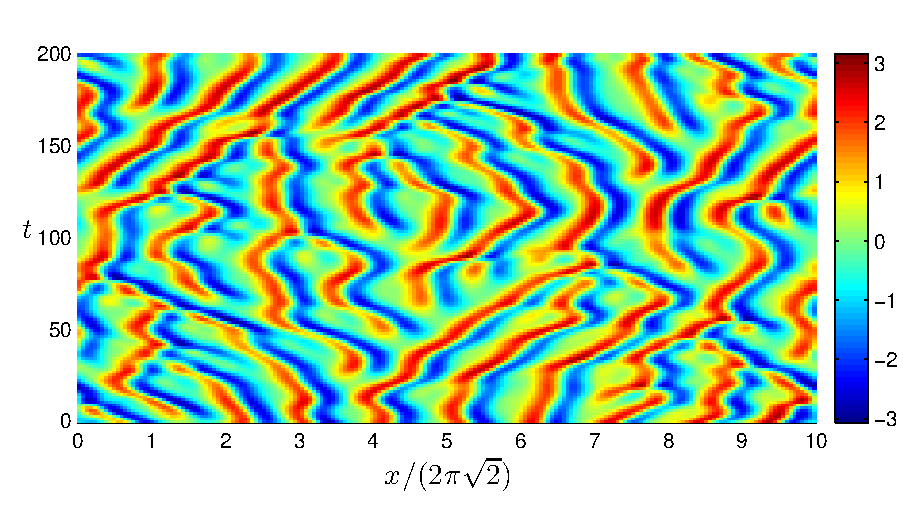
\includegraphics[width=0.9\textwidth]{figs_bmp/ks_largeL_cbar_200.eps} 
\end{center}
\caption{
A typical spatiotemporally chaotic solution of the \KSe, system size
$L=20\pi\sqrt{2}\approx 88.86$.  The $x$ coordinate is scaled
with the most unstable wavelength $2\pi\sqrt{2}$, which is
approximately also the mean wavelength of the turbulent flow.
The color bar indicates the color scheme for $u(x,t)$, used also
for the subsequent figures of this type.
     } \label{f:ks_largeL}
\end{figure}
%%%%%%%%%%%%%%%%%%%%%%%%%%%%%%%%%%%%%%%%%%%%%%%%%%%%%%%%%%%%%%%%%%

\subsection{Symmetries of \KSe}
\label{sec:KSeSymm}

The KS equation is Galilean invariant: if $u(x,t)$ is a solution,
then $u(x -ct,t) -c $, with $c$ an arbitrary constant
speed, is also a solution. Without loss of generality, in our
calculations we shall set the mean velocity of the front to zero,
\beq \int dx \, u = 0 \,. \ee{GalInv}
As $\dot{a_0}=0$ in
\refeq{expan}, $a_0$ is a conserved quantity
fixed to $a_0=0$ by the condition \refeq{GalInv}. $G$, the group of actions $ g \in G $ on a
\statesp\ (reflections, translations, \etc) is a symmetry of the KS
flow \refeq{ks} if $g\,u_t = F(g\,u)$.
The KS equation is time translationally invariant, and space translationally invariant
on a periodic domain under
the 1-parameter group of
$O(2): \{\Shift_{\shift/L},\Refl \}$.
If $u(x,t)$ is a solution, then
$\Shift_{\shift/L}\, u(x,t) = u(x+\shift,t)$
is an equivalent solution for any shift
$-L/2 < \shift \leq L/2$,
as is the
reflection (`parity' or `inversion')
\beq
    \Refl \, u(x) = -u(-x)
\,.
\ee{KSparity}
The translation operator action on the Fourier coefficients \refeq{eq:ksexp},
represented here by a complex valued vector
$a = \{a_k\in\mathbb{C}\,|\,k = 1, 2, \ldots\}$, is given by
\beq
  \Shift_{\shift/L}\, a = \mathbf{g}(\shift) \, a \,,
  \label{eq:shiftFour}
\eeq
where $\mathbf{g}(\shift) = \diag( e^{i q_k\, \shift} )$ is a complex
valued diagonal matrix, which amounts to the $k$-th mode complex plane
rotation by an angle $k\, \shift /\tildeL$.  The reflection acts on
the Fourier coefficients by complex conjugation,
\beq
  \Refl \, a = -a^\ast
\,.
\ee{FModInvSymm}
Reflection generates the dihedral subgroup $D_1 = \{1, \Refl\}$
of $O(2)$.  Let $\bbU$ be the space of
real-valued velocity fields periodic and square integrable
on the interval $\Omega = [-L/2,L/2]$,
\begin{align}
 \bbU  &= \{u \in L^2(\Omega) \; | \; u(x) = u(x+L)\}  \,.
\end{align}
A continuous symmetry maps each state $u \in \bbU$
to a manifold of functions with identical dynamic behavior.
Relation $\Refl^2 = 1$ induces linear decomposition
$u(x) = u^+(x)+ u^-(x)$,
$u^\pm(x)= P^\pm u(x) \in  \bbU^\pm$,
into irreducible subspaces
$
\bbU = \bbU^+
       \oplus \bbU^-
$, where
\beq
    P^+=(1+\Refl)/2
    \,,\qquad
    P^-=(1-\Refl)/2
\,,
\ee{P1P2proj} are the antisymmetric/symmetric projection operators.
Applying $P^+,\,P^-$ on the KS equation \refeq{ks} we have\rf{KNSks90}
\bea
 u_t^+ &=& - (u^+u^+_x + u^-u^-_x )
                - u^+_{xx} - u^+_{xxxx}
    \continue
 u_t^- &=& - (u^+u^-_x + u^-u^+_x )
                - u^-_{xx} - u^-_{xxxx}
\,.
\label{KSD1}
\eea
If $u^- = 0$, KS flow is confined to
the antisymmetric $\bbU^+$ subspace,
\beq
 u_t^+ = - u^+u^+_x
                - u^+_{xx} - u^+_{xxxx}
\,,
\label{KSU+}
\eeq
but otherwise the nonlinear terms in \refeq{KSD1}
mix the two subspaces.

Any rational shift $ \Shift_{1/m}u(x)=u(x+L/m)$ generates a discrete
cyclic subgroup $C_m$ of $O(2)$, also a symmetry of KS
system. Reflection together with $C_m$ generates another
symmetry of KS system, the dihedral subgroup $D_m$ of $O(2)$.
The only non-zero Fourier components of a solution invariant
under $C_m$ are $a_{jm} \neq 0$, $j =1,2,\cdots$, while for a
solution invariant under $D_m$ we also have the condition
$\Re a_j=0$ for all $j$.
$D_m$ reduces the dimensionality of \statesp\ and aids computation of
\eqva\ and \po s within it. For example, the 1/2-cell translations \beq
    \Shift_{1/2}\, u(x)=u(x+L/2)
\ee{KSshift}
and reflections generate $O(2)$
subgroup $D_2 = \{1, \Refl,\Shift,\Shift\Refl\}$,
which
reduces the \statesp\ into four irreducible subspaces
(for brevity, here $\Shift = \Shift_{1/2}$):
\begin{align}
 & \qquad\qquad\qquad\qquad\qquad
              ~~~ \Shift ~~ \Refl  ~\;  \Shift\Refl
    \nnu\\
P^{(1)} &= \frac{1}{4} (1 + \Shift + \Refl + \Shift\Refl)
           ~~~~  S  ~~  S   ~~   S
    \nnu\\
P^{(2)} &= \frac{1}{4} (1 + \Shift - \Refl - \Shift\Refl)
            ~~~~  S  ~~  A   ~~   A
    \nnu\\
P^{(3)} &= \frac{1}{4} (1 - \Shift + \Refl - \Shift\Refl)
           ~~~~  A  ~~  S   ~~   A
     \label{ek_defn}\\
P^{(4)} &= \frac{1}{4} (1 - \Shift - \Refl + \Shift\Refl)
          ~~~~  A  ~~  A   ~~   S
\,.
    \nnu
\end{align}
$P^{(j)}$ is the projection operator onto
$u^{(j)}$ irreducible subspace, and the last 3 columns
refer to the symmetry (or antisymmetry) of
$u^{(j)}$ functions under reflection and
1/2-cell shift.
By the same argument that identified \refeq{KSU+} as
the invariant subspace of KS, here the KS flow
stays within the
 $\bbU^S =  \bbU^{(1)}+ \bbU^{(2)}$
irreducible $D_1$ subspace of
$u$ profiles symmetric under 1/2-cell shifts.

While in general the bilinear term $(u^2)_x$  mixes the
irreducible subspaces of $D_n$, for $D_2$ there are
four subspaces invariant under the flow\rf{KNSks90}:
\begin{romannum}
 \item[$\{0\}$:~~~~~~] the $u(x)=0$ {\eqv}
 \item[$\bbU^+ = \bbU^{(1)}+ \bbU^{(3)} $:]
    the reflection $D_1$ irreducible space of antisymmetric $u(x)$
 \item[$\bbU^S =  \bbU^{(1)}+ \bbU^{(2)}$:]
    the shift $D_1$ irreducible space of $L/2$ shift symmetric  $u(x)$
 \item[$\bbU^{(1)}$:~~~~~]
    the $D_2$ irreducible  space of $u(x)$ invariant under $x\mapsto L/2-x,\ u\mapsto -u$.
\end{romannum}
With the continuous
translational symmetry eliminated within each subspace, there are no
\reqva\ and \rpo s, and one
can focus on the \eqva\ and \po s only, as was done
for $\bbU^+$ in \refrefs{Christiansen97,LanThesis,lanCvit07}.
In the Fourier
representation, the
$u \in \bbU^+$
antisymmetry amounts to having purely imaginary
coefficients, since $a_{-k}= a^\ast_k = -a_k$.
The 1/2 cell-size shift $\Shift_{1/2}$
generated 2-element discrete subgroup
$\{1,\Shift_{1/2}\}$ is
of particular interest
because in the $\bbU^+$ subspace the translational invariance of the full system reduces to
invariance under discrete translation \refeq{KSshift} by half a
spatial period $L/2$.

Each of the above dynamically invariant subspaces is unstable
under small perturbations, and generic solutions of \KSe\ belong to
the full space.
Nevertheless, since  all \eqva\ of the KS flow studied in this paper
lie in the $\bbU^+$ subspace (see
\refsect{sec:L22}), $\bbU^+$  plays important role for the global
geometry of the flow.
The linear stability matrices of these \eqva\ have
eigenvectors both in and outside of $\bbU^+$, and need to be
computed in the full \statesp.




\subsection{\Eqva\ and \reqva}
\label{sec:stks}

\Eqva\  (or the steady solutions)
are the fixed profile time-invariant solutions,
\beq
 u(x,t) = u_\stagn(x)
\,.
\ee{eqva}
Due to the translational symmetry,
the KS system also allows for
\reqva\ (traveling waves, rotating waves),
characterized by a fixed profile $u_\stagn(x)$
moving with constant speed $c$, {\ie}
\beq
 u(x,t) =  u_\stagn(x-ct)
\,.
\ee{reqva}
Here suffix ${}_\stagn$ labels a particular invariant solution.
Because of the reflection symmetry \refeq{KSparity},
the \reqva\ come in counter-traveling pairs
$u_\stagn(x-ct)$, $-u_\stagn(-x+ct)$.

The \reqv\ condition for the {\KS} PDE \refeq{ks}
is the ODE
\beq
{\textstyle\frac{1}{2}}(u^2)_x+u_{xx}+ u_{xxxx}=c \, u_x
\ee{KSeqvCond}
which can be analyzed as a dynamical system in its own right.
Integrating once we get
\beq
{\textstyle\frac{1}{2}}u^2 - c u + u_x + u_{xxx}=\expctE
\,.
\label{eq:stdks}
\eeq
This equation can be interpreted as a 3-dimen\-si\-on\-al dynamical system
with spatial coordinate $x$ playing the role of `time,'
and the integration constant \expctE\ can be interpreted as `energy,'
see \refsect{sec:energy}.

For $\expctE>0$ there is rich $\expctE$-dependent dynamics,
with fractal sets of bounded solutions investigated in depth
by Michelson\rf{Mks86}. For $\tildeL<1$ the only \eqv\ of the
system is the globally attracting constant solution
$u(x,t)=0$, denoted $\EQV{0}$ from now on. With increasing
system size $L$ the system undergoes a series of
bifurcations. The resulting \eqva\ and \reqva\ are described
in the classical papers of Kevrekidis, Nicolaenko and
Scovel\rf{KNSks90}, and Greene and Kim\rf{ksgreene88},
among others. The relevant bifurcations up to the
system size investigated here are summarized in
\reffig{fig:ksBifDiag}: at $\tildeL=22/2\pi = 3.5014\cdots$,
the {\eqva} are the constant solution \EQV{0},
the  \eqv\ \EQV{1} called GLMRT by Greene and
Kim\rf{laquey74,ksgreene88},
the $2$- and $3$-cell states
\EQV{2} and \EQV{3}, and the pairs of \reqva\ \REQV{\pm}{1},
\REQV{\pm}{2}.
All \eqva\ are in the antisymmetric subspace $\bbU^+$, while
\EQV{2} is also invariant under $D_2$ and \EQV{3} under
$D_3$.


%%%%%%%%%%%%%%%%%%%%%%%%%%%%%%%%%%%%%%%%%%%%%%%%%%%%%%%%%%%%%%%%
\begin{figure}[t]       \label{fig:ksBifDiag}
\begin{center}
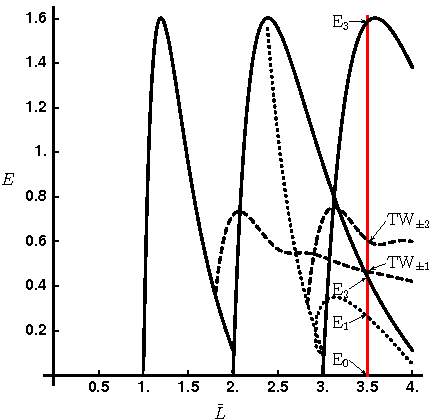
\includegraphics[width=0.5\textwidth]{figs_bmp/ksBifDiag_pst.eps}
\end{center}
\caption{
The energy \refeq{ksEnergy} of the \eqva\ and \reqva\ that
exist up to $L=22$, $\tildeL = 3.5014\ldots$, plotted as a function
of the system size $\tildeL = L/2\pi$ (additional \eqva, not present
at $L = 22$ are given in \refref{ksgreene88}). Solid curves denote
$n$-cell solutions \EQV{2} and \EQV{3}, dotted curves the GLMRT
\eqv\ \EQV{1},
and dashed curves the \reqva\ \REQV{\pm}{1} and \REQV{\pm}{2}.
The parameter $\alpha$ of \refrefs{KNSks90,ksgreene88} is
related to the system size by $\tildeL=\sqrt{\alpha/4}$.
        }
\end{figure}
%%%%%%%%%%%%%%%%%%%%%%%%%%%%%%%%%%%%%%%%%%%%%%%%%%%%%%%%%%%%%%%%%%

In the Fourier representation the \reqva\ time dependence is
\beq
 a_k(t) e^{-itc q_k} = a_k(0)
\,.
\ee{reqvaF}
Differentiating with respect to time, we obtain
the Fourier space version of the \reqv\ condition
\refeq{KSeqvCond},
\beq
 \pVeloc_k(a) - i q_k \velRel a_k = 0
\,,
\ee{reqvCondF}
which we solve for (time independent) $a_k$ and $c$.
Periods of spatially periodic {\eqva} are $L/n$ with integer $n$.
Every time the system size crosses  $\tildeL=n$,
$n$-cell states
are generated through pitchfork bifurcations off $u =0$
equilibrium.
Due to the translational invariance of {\KSe},
they form invariant circles
in the full \statesp.
In the $\bbU^+$ subspace considered here,
they correspond to $2n$ points, each shifted by $L/2n$.
For a sufficiently small $L$
the number of {\eqva} is small and
concentrated on the low wave-number end of the Fourier spectrum.

In a periodic box of size $L$
both \eqva\ and \reqva\ are  periodic solutions
embedded in 3-$d$ space, conveniently represented as loops in
$(u,u_x,u_{xx})$ space, see \reffig{f:KS22Equil}\,(\textit{d}).
In this representation the continuous translation symmetry
is automatic -- a rotation in the $[0,L]$ periodic domain only
moves the points along the loop. For an \eqv\ the points
are stationary in time; for \reqv\ they move in time, but in
either case, the loop remains invariant.
So we do not have the problem that we encounter in the Fourier
representation, where seen from the frame of one of the \eqva\
the rest trace out circles under the action of continuous symmetry
translations.

From \refeq{expan} we see that the origin $u(x,t) = 0$
has Fourier modes as the linear stability eigenvectors
(see \refappe{sec:stability}).  The $|k|<\tildeL$
long wavelength perturbations of the flat-front {\eqv}
are linearly unstable, while for
$|k|$ sufficiently larger than $\tildeL$ the short wavelength
perturbations are strongly contractive. The high $k$
eigenvalues, corresponding to rapid variations of the flame
front, decay so fast that the corresponding eigendirections
are physically irrelevant. Indeed, \refref{YaTaGiChRa08} shows that
the chaotic solutions of spatially extended dissipative
systems evolve within an inertial manifold spanned by a
finite number of physical modes, hyperbolically isolated from
a set of residual degrees of freedom with high $k$, themselves individually
isolated from each other.
The most unstable mode, nearest to $|k|=\tildeL/\sqrt{2}$,
sets the scale of the mean wavelength $\sqrt{2}$
of the KS `turbulent' dynamics,
see \reffig{f:ks_largeL}.


\subsection{\Rpo s, symmetries and \po s} \label{sec:KSePO}

The KS equation \refeq{ks} is time translationally invariant, and
space translationally invariant under the 1-$d$ Lie group of $O(2)$
rotations: if $u(x,t)$ is a solution, then $u(x+\shift,t)$ and
$-u(-x,t)$ are equivalent solutions for any $-L/2 < \shift \leq
L/2$.
As a result of invariance under $\Shift_{\shift/L}$,
KS equation can have \rpo\ solutions
with a profile $u_p(x)$, period $\period{p}$, and a
nonzero shift $\shift_p$
\beq
  \Shift_{\shift_p/L}u(x,\period{p}) =
  u(x+\shift_p,\period{p}) = u(x,0) = u_p(x)\,.
\label{KSrpos}
\eeq
{\Rpo s} \refeq{KSrpos} are periodic in
$\velRel_p=\shift_p/\period{p}$ co-rotating frame (see
\reffig{f:MeanVelocityFrame}), but in the stationary frame their
trajectories are quasiperiodic.  Due to the reflection symmetry
\refeq{KSparity} of KS equation, every {\rpo} $u_p(x)$ with shift
$\shift_p$ has a symmetric partner $-u_p(-x)$ with shift $-\shift_p$.

Due to invariance under reflections, KS equation can also have
\rpo s {\em with reflection}, which are
characterized by a profile $u_p(x)$ and
period $\period{p}$
\beq
  \Refl u(x+\shift,\period{p}) =
  -u(-x-\shift,\period{p}) = u(x+\shift,0) = u_p(x)
  \,,
\label{KSpos}
\eeq
giving the family of equivalent solutions
parameterized by $\shift$
(as the choice of the reflection point is arbitrary,
the shift can take any value in $-L/2 < \shift \leq L/2$).

Armbruster \etal\rf{AGHks89,AGHO288} and Brown and
Kevrekidis\rf{BrKevr96} (see also \refref{Krupa90}) link the
birth of \rpo s to an infinite period global bifurcation
involving a heteroclinic loop connecting equilibria or a
bifurcation of \reqva, and also report creation of \rpo\
branches through bifurcation of \po s.

As $\shift$ is continuous in the interval $[-L/2, L/2]$,
the likelihood of a \rpo\ with $\shift_p = 0$ shift is zero,
unless an exact periodicity is enforced by a discrete symmetry,
such as the dihedral symmetries discussed above.
If the shift $\shift_p$ of a \rpo\ with period $\period{p}$ is such
that $\shift_p /L$ is a rational number, then the orbit is
periodic with period $n\period{p}$.  The likelihood to find such \po s is
also zero.

However, due to the KS equation invariance under
the dihedral $D_n$ and cyclic $C_n$ subgroups, the following
types of \po s are possible:

{\bf (a)} The \po\ lies
within a subspace pointwise invariant under the action of
$D_n$ or $C_n$. For instance, for $D_1$ this is the
$\bbU^+$ antisymmetric subspace, $-u_p(-x) = u_p(x)$, and
$u(x,\period{p}) = u(x,0) = u_p(x)$. The periodic orbits
found in \refrefs{Christiansen97,lanCvit07} are
all in $\bbU^+$, as the dynamics is restricted to
antisymmetric subspace. For $L=22$ the dynamics in $\bbU^+$
is dominated by attracting (within the subspace)
heteroclinic connections and thus we have no periodic orbits
of this type, or in any other of the $D_n$--invariant
subspaces, see \refsect{sec:L22}.

{\bf (b)} The \po\ satisfies
\beq
	 u(x,t+\period{p})=\gamma u(x,t)\,,
	\label{eq:POspattemp}
\eeq
for some group element $\gamma\in O(2)$ such that
$\gamma^m=e$ for some integer $m$ so that the orbit repeats
after time $m \period{p}$ (see
\refref{golubitsky2002sp} for a general discussion of
conditions on the symmetry of a \po).
If an orbit is of reflection type \refeq{KSpos},
$\Refl\Shift_{\shift/L} u(x,\period{p}) =
-u(-x-\shift,\period{p}) = u(x,0)$, then it is pre-periodic
to a \po\ with period $2\period{p}$. Indeed, since
$(\Refl\Shift_{\shift/L})^2 = \Refl^2 = 1$, and the KS
solutions are time translation invariant, it follows from
\refeq{KSpos} that
\[
  u(x,2\period{p}) = \Refl\Shift_{\shift/L} u(x,\period{p}) =
  (\Refl\Shift_{\shift/L})^2 u(x,0) = u(x,0)\;.
\]
Thus any shift acquired during time $0$ to
$\period{p}$ is compensated by the opposite shift during
evolution from $\period{p}$ to $2 \period{p}$.
All periodic orbits we have found for $L=22$ are of type
\refeq{eq:POspattemp} with $\gamma=R$. Pre-periodic orbits
with $\gamma\in C_n$ have been found by Brown and
Kevrekidis\rf{BrKevr96} for KS system sizes larger than ours,
but we have not found any for $L=22$.
Pre-periodic orbits are a hallmark of any dynamical system
with a discrete symmetry, where they have a natural
interpretation as \po s in the fundamental
domain\rf{CvitaEckardt,DasBuch}.

\section{Energy transfer rates}
\label{sec:energy}

In physical settings where the observation times are much
longer than the dynamical `turnover' and Lyapunov times
(statistical mechanics, quantum physics, turbulence) periodic
orbit theory\rf{DasBuch} provides highly accurate predictions
of measurable long-time averages such as the dissipation and
the turbulent drag\rf{GHCW07}. Physical predictions have to
be independent of a particular choice of ODE representation
of the PDE under consideration and, most importantly,
invariant under all symmetries of the dynamics. In this
section we discuss a set of such physical observables for the
1-$d$ KS invariant under reflections and translations. They
offer a representation of dynamics in which the symmetries
are explicitly quotiented out. We shall use these
observables in \refsect{sec:energyL22} in order to
visualize a set of solutions on these coordinates.

The {space average} of a function $\obser = \obser(\pSpace,t) = \obser(u(x,t))$  on
the interval $L$,
\beq
    \expct{\obser} = \Lint{\pSpace}\, \obser(\pSpace,t)
    \,,
    \label{rpo:spac_ave}
\eeq
is in general time dependent.
Its mean value is given by the {time average}
\beq
\timeAver{\obser}
    =
\lim_{t\rightarrow \infty} \frac{1}{t} \int_0^t \! d\tau \, \expct{\obser}
    =
\lim_{t\rightarrow \infty} \frac{1}{t} \int_0^t \!
    \Lint{\tau}  d\pSpace\, \obser(\pSpace,\tau)
    \,.
\label{rpo:tim_ave}
\eeq
The mean value of $\obser = \obser(u_\stagn) \equiv \obser_\stagn$ evaluated on
\eqv\ or {\reqv} $u(\pSpace,t) = u_\stagn(\pSpace-ct)$, labeled by  $q$ as in 
\refeq{reqva}, is
\beq
\timeAver{\obser}_\stagn = \expct{\obser}_\stagn = \obser_\stagn\,.
\label{rpo:u-eqv} \eeq 
Evaluation of the infinite time average
\refeq{rpo:tim_ave} on a function of a \po\ or \rpo\
$u_p(\pSpace,t)=u_p(\pSpace+\shift_p,t+\period{p})$ requires only a single
$\period{p}$ traversal,
\beq
  \timeAver{\obser}_p = \frac{1}{\period{p}}
    \int_0^{\period{p}} \! d\tau \, \expct{\obser}
\,.
\label{rpo:u-cyc}
\eeq

Equation \refeq{ks} can be written as
\beq
    u_t=- V_x
        \,,\qquad
    V(x,t)={\textstyle\frac{1}{2}}u^2+u_{x} + u_{xxx}
    \,.
\ee{ksPotent}
If $u$ is `flame-front velocity' then \expctE, defined in
\refeq{eq:stdks}, can be interpreted as the mean energy
density. So, even though KS is a phenomenological
small-amplitude equation, the time-dependent $L^2$ norm
of $u$,
\beq
    \expctE=
  \Lint{\pSpace}
  V(x,t)=
  \Lint{\pSpace} \frac{u^2}{2}
  \,,
  \label{ksEnergy}
\eeq
has a physical interpretation\rf{ksgreene88} as the average `energy'
density of the flame front. This analogy to the mean kinetic energy
density for the Navier-Stokes motivates what follows.

The energy \refeq{ksEnergy} is intrinsic to the flow,
independent of the particular ODE basis set chosen to
represent the PDE. However, as the Fourier amplitudes are
eigenvectors of the translation operator, in the Fourier
space the energy is a diagonalized quadratic norm,
\beq
\expctE
          =  \sum_{k=-\infty}^{\infty} E_k
\,,\qquad
E_k =
    {\textstyle\frac{1}{2}}|a_k|^2
\,,
\ee{EFourier}
and explicitly invariant term by term
under translations
\refeq{eq:shiftFour}
and reflections \refeq{KSparity}.

Take time derivative of the energy density \refeq{ksEnergy},
substitute \refeq{ks} and integrate by parts. Total derivatives vanish
by the spatial periodicity on the $L$ domain:
\bea
   \dot{\expctE} &=&
     \expct{u_t \, u}
         = - \expct{\left({u^2}/{2} + u_{x} + u_{xxx}\right)_x u }
    \continue
    &=&
\expct{ u_x \, {u^2}/{2} + u_{x}^2 + u_x \, u_{xxx}}
    \,.
\label{rpo:ksErate}
\eea
The first term in \refeq{rpo:ksErate} vanishes by
integration by parts,
\(
3 \expct{ u_x \, u^2}= \expct{(u^3)_x} = 0
\,,
\)
and integrating the third term by parts yet again
one gets\rf{ksgreene88} that the energy variation
\beq
   \dot{\expctE} = P - D
                \,,\qquad
      P =  \expct{u_{x}^2}
                \,,\quad
      D =  \expct{u_{xx}^2}
\ee{EnRate}
balances the power $P$ pumped in by anti-diffusion $u_{xx}$
against the energy dissipation rate $D$
by hyper-viscosity $u_{xxxx}$
in the KS equation \refeq{ks}.

The time averaged energy density  $\timeAver{E}$
computed on a typical orbit goes to a constant, so
the mean values \refeq{rpo:tim_ave} of drive and dissipation
exactly balance each other:
\beq
    \timeAver{\dot{E}}  =
    \lim_{t\rightarrow \infty}
        \frac{1}{t} \int_0^t d\tau \, \dot{\expctE}
=
      \timeAver{P} - \timeAver{D}
= 0
    \,.
\ee{rpo:EtimAve}
In particular, the \eqva\
and \reqva\ fall onto the diagonal in \reffig{f:drivedrag}\,(\textit{a}),
and so do time averages computed on \po s and \rpo s:
\beq
\timeAver{E}_p =
\frac{1}{\period{p}} \int_0^\period{p}d\tau \, E(\tau)
    \,,\qquad
\timeAver{P}_p =
\frac{1}{\period{p}} \int_0^\period{p} d\tau \, P(\tau)
    =
      \timeAver{D}_p
    \,.
\label{poE}
\eeq
In the Fourier basis \refeq{EFourier} the conservation of energy on average
takes form
\beq
0 = \sum_{k=-\infty}^{\infty} ( q_k^2 - q_k^4 )\,
    \timeAver{E}_k
\,,\qquad
E_k(t) =  {\textstyle\frac{1}{2}} |a_k(t)|^2
\,.
\ee{EFourier1}
The large $k$ convergence of this series is insensitive to the
system size $L$; $\timeAver{E_k}$ have to decrease much faster than
$q_k^{-4}$.
Deviation of $E_k$ from this bound for small $k$ determines the active modes.
For \eqva\ an $L$-independent bound
    on $E$ is given by Michelson\rf{Mks86}.
The best current bound\rf{GiacoOtto05,bronski2005} on the long-time limit
of $E$
as a function of the system size $L$ scales as
$E \propto L^2$.

% L22eqv.tex
% $Author: siminos $ $Date: 2009-10-01 17:27:03 -0400 (Thu, 01 Oct 2009) $

\section{Geometry of state space with $L=22$}
\label{sec:L22}

%%%%%%%%%%%%%%%%%%%%%%%%%%%%%%%%%%%%%%%%%%%%%%%%%%%%%%%%%%%%%%
\begin{figure}[t]
\begin{center}
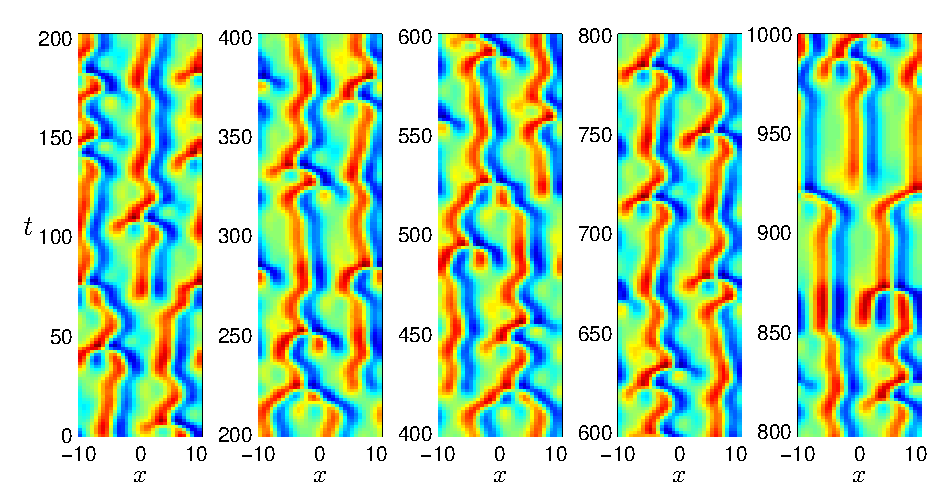
\includegraphics[width=0.9\textwidth, clip=true]{figs/ks_L22_long_orbit.eps}
\end{center}
\caption{
A typical chaotic orbit of the KS flow, system size $L=22$.
     } \label{f:ks_L22}
\end{figure}
%%%%%%%%%%%%%%%%%%%%%%%%%%%%%%%%%%%%%%%%%%%%%%%%%%%%%%%%%%%%%%%%%%
We now turn to exploring Hopf's vision
numerically, on a specific KS system.
An instructive example is offered by the dynamics for
the  $L=22$  system
that we specialize to for the rest of this paper.
The size of this
small system is $\sim 2.5$ mean wavelengths
($\tildeL/\sqrt{2}= 2.4758\ldots$),
and the competition between states with wavenumbers 2 and 3
leads to
what, in the context of boundary shear flows, would be
called\rf{HaKiWa95} the `empirically observed sustained
turbulence,' but in the present context may equally well be
characterized as a `chaotic attractor.' A typical long orbit
is shown in \reffig{f:ks_L22}.
Asymptotic attractor structure of small systems like
the one studied here
is very sensitive to system parameter variations, and,
as is true of
any realistic unsteady flow, there is no rigorous way of
establishing that this `turbulence' is sustained for all time,
rather than being
merely a very long transient on a way to an
attracting periodic state.
For large system size, as the one shown in \reffig{f:ks_largeL}, it is
hard to imagine a scenario under which attracting periodic states
(as shown in \refref{FSTks86}, they do exist) would have significantly
large immediate basins of attraction.
Regardless of the
(non)existence of a $t \to \infty$ chaotic attractor, study
of the invariant unstable solutions and the associated Smale
horseshoe structures in system's \statesp\ offers valuable
insights into the observed unstable `coherent structures.'

Because of the strong $k^4$ contraction, for a small system
size the long-time dynamics
is confined to low-dimensional
inertial manifold\rf{jolly_evaluating_2000}.
Indeed, numerically the covariant Lyapunov vectors\rf{ginelli-2007-99} of the
$L=22$ chaotic attractor separate into 8 ``physical''
vectors with small Lyapunov exponents
$(\Lyap_j) = (0.048,$ 0, 0, $-0.003$, $-0.189$, $-0.256$,
$-0.290$, $-0.310$),
and the remaining 54 ``hyperbolically isolated'' vectors
with rapidly decreasing exponents
$(\Lyap_j) = (-1.963$,   $-1.967$,   $-5.605$,   $-5.605$,  $-11.923$,  $-11.923$,
 $\cdots) \approx -(j/\tildeL)^4$,
in full agreement with the Yang \etal\rf{YaTaGiChRa08}
investigations of KS for large systems sizes.
%, up to $L=192$.
The chaotic dynamics mostly takes place close to a
8-dimensional manifold, with strong contraction in other
dimensions.  The two zero exponents are due to the time and
space translational symmetries of the \KSe\ and the 2 corresponding
dimensions can be quotiented out by means of discrete-time
Poincar\'e sections and $O(2)$ group orbit slices.
It was shown
in \refrefs{Christiansen97,lanCvit07} that within unstable-manifold
curvilinear coordinate frames, the dynamics on the attractor
can sometimes be well approximated by local 1- or 2-dimensional
Poincar\'e return maps.
Hence a relatively small number of real Fourier modes, such as 62
to 126 used in calculations presented here, suffices
to obtain  invariant
solutions numerically accurate to within $10^{-5}$.

We next investigate the properties of \eqva\ and \reqva\ and
determine numerically a large set of the short periods \rpo s
for KS in a periodic cell of size $L=22$.

\section{\Eqva\ and \reqva\ for $L=22$}

In addition to the trivial \eqv\ $u=0$ (denoted \EQV{0}),
we find three \eqva\ with dominant wavenumber $k$
(denoted \EQV{k}) for $k = 1, 2, 3$.  All {\eqva}, shown in
\reffig{f:KS22Equil}, are symmetric with respect to the reflection
symmetry \refeq{KSparity}.
In addition, \EQV{2} and \EQV{3} are symmetric with respect
to translation \refeq{KSshift}, by $L/2$ and $L/3$, respectively.
\EQV{2} and \EQV{3} essentially lie in
the 2$^\mathrm{nd}$ and 3$^\mathrm{rd}$ Fourier component complex planes,
with small  deformations of the $k=2j$ and $k=3j$ harmonics, respectively.

%%%%%%%%%%%%%%%%%%%%%%%%%%%%%%%%%%%%%%%%%%%%%%%%%%%%%%%%%%%%%%%%%%
\begin{figure}[t]
\begin{center}
  (\textit{a})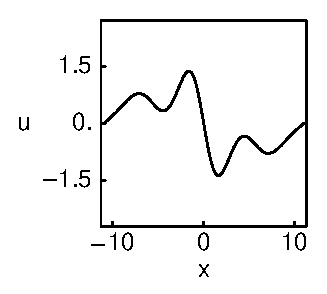
\includegraphics[width=0.35\textwidth, clip=true]{figs/1wKS22equil.eps}
~~~~(\textit{b})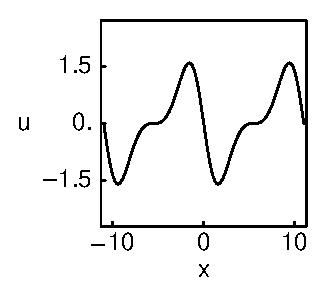
\includegraphics[width=0.35\textwidth, clip=true]{figs/2wKS22equil.eps}
\\
  (\textit{c})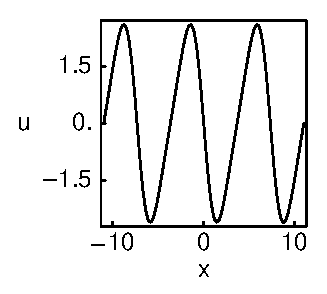
\includegraphics[width=0.35\textwidth, clip=true]{figs/3wKS22equil.eps}
~~~~(\textit{d})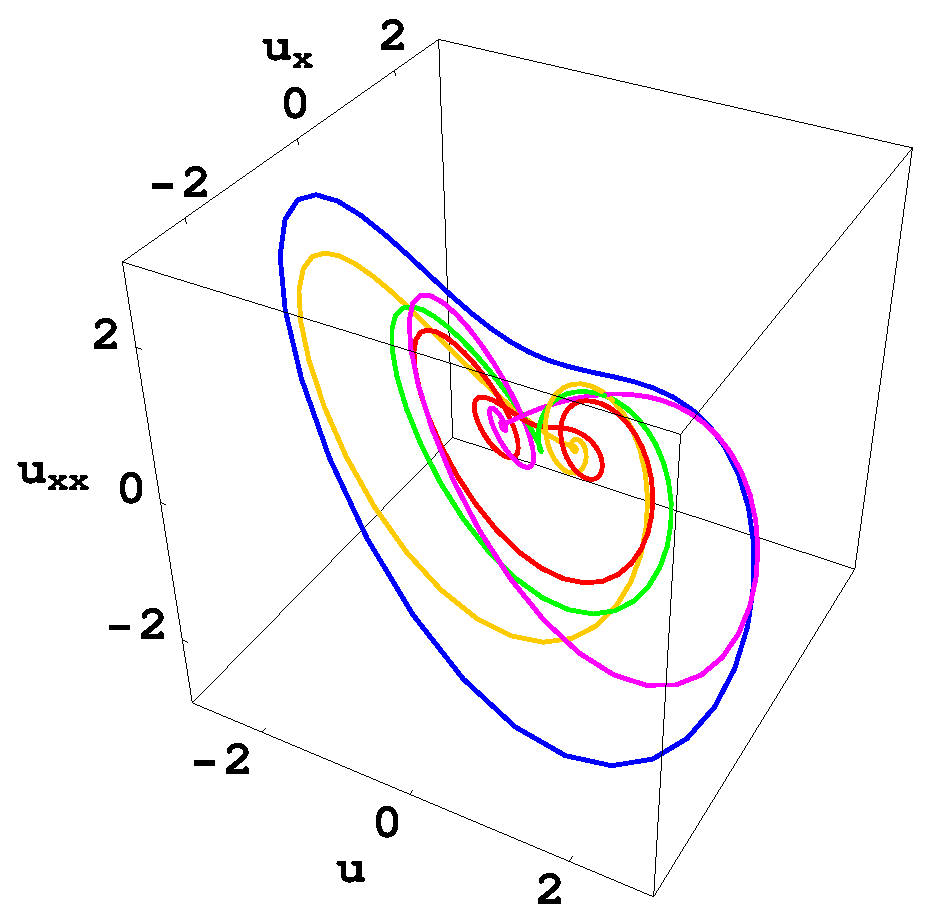
\includegraphics[width=0.35\textwidth, clip=true]{figs/equilSpatial.eps}
\end{center}
\caption{
(a) \EQV{1}, (b) \EQV{2}, and (c)
\EQV{3} \eqva. The \EQV{0} \eqv\ is the $u(x)=0$ solution.
(d) $(u,u_x,u_{xx})$ representation
of (red) \EQV{1}, (green) \EQV{2},  (blue) \EQV{3} \eqva,
(purple) \REQV{+}{1},  and (orange) \REQV{-}{1} \reqva.
$L=22$ system size.
    }
\label{f:KS22Equil}
\end{figure}
%%%%%%%%%%%%%%%%%%%%%%%%%%%%%%%%%%%%%%%%%%%%%%%%%%%%%%%%%%%%%%%%

The stability of the {\eqva} is characterized by the eigenvalues
$\eigExp[j]$ of the \stabmat.  The leading 10 eigenvalues for each
\eqv\ are listed in \reftab{tab:Eksym};
those with $\eigRe > -2.5$ are also plotted in
\reffig{f:KS22EkEigs}.
We have computed (available upon request) the corresponding
eigenvectors as well. As an \eqv\ with $\mathrm{Re}\,
\Lyap_j > 0$ is unstable in the direction of the
corresponding eigenvector $\jEigvec{j}$, the eigenvectors
provide flow-intrinsic (PDE discretization independent)
coordinates which we use for visualization of unstable
manifolds and homo/heteroclinic connections between \eqva.
We find such coordinate frames, introduced by
Gibson \etal\rf{GHCW07,GibsonMovies}, better suited to visualization
of nontrivial solutions than the more standard Fourier mode
(eigenvectors of the $u(x,t)=0$ solution) projections.


The eigenvalues of \EQV{0} are determined by the linear part of the KS
equation \refeq{expanMvar}: $\Lyap_k=(k/\tilde{L})^2-(k/\tilde{L})^4$.
For $L=22$, there are three pairs of unstable eigenvalues, corresponding,
in decreasing order, to three unstable modes $k=2,3$, and 1.  For each
mode, the corresponding eigenvectors lie in the plane spanned by
$\Re \, a_k$ and $\Im \, a_k$. \refTab{tab:Eksym}
lists the symmetries of the stability eigenvectors of
\eqva\ \EQV{1} to \EQV{3}.

\begin{figure}[t]
\begin{center}
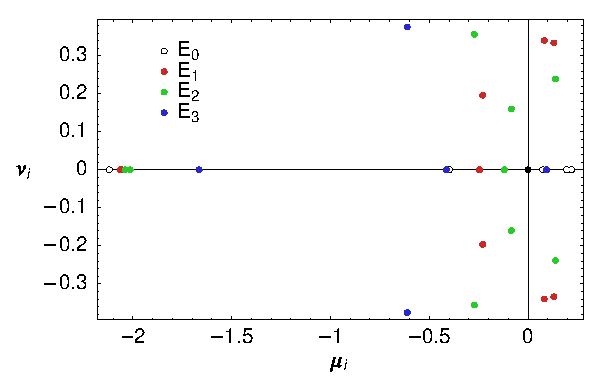
\includegraphics[width=4in]{figs/L22-eqvaEigenvalues.eps}
\end{center}
\caption{
Leading  \eqv\ stability eigenvalues,
$L=22$ system size.
}
\label{f:KS22EkEigs}
\end{figure}

\begin{table}[t]
\caption{
Leading eigenvalues
$\eigExp[j]= \eigRe[j] \pm i\eigIm[j]$
and symmetries of the corresponding eigenvectors
of KS {\eqva} and \reqva\ for $L = 22$ system size.
We have used as our reference states the ones that lie within
the antisymmetric subspace  $\bbU^+$,
and also listed the symmetries of
the $L/4$ translated ones.
        }\label{tab:Eksym}
\begin{center} \footnotesize
\begin{tabular}{ccccc}
\EQV{1}& $\eigRe[j]$ & $\eigIm[j]$ & Symmetry & $\Shift_{1/4}\EQV{n}$ Symmetry\\\hline
  $\eigExp[1,2]$ & $\ \ 0.1308$& $0.3341$ & -  & -\\
  $\eigExp[3,4]$ & $\ \ 0.0824$& $0.3402$ & $\bbU^+$  & $\bbU^{(1)}$\\
  $\eigExp[5]$   & $0$     &          & -  & -\\
  $\eigExp[6,7]$ &$-0.2287$& $0.1963$ & $\bbU^+$  & $\bbU^{(1)}$\\
  $\eigExp[8]$   &$-0.2455$&          & -  & -\\
  $\eigExp[9]$   &$-2.0554$&          & $\bbU^+$  & $\bbU^{(1)}$\\
  $\eigExp[10]$  &$-2.0619$&          & -  & -\\[2ex]
\EQV{2}&  &  & \\\hline
  $\eigExp[1,2]$ & $\ \ 0.1390$& $0.2384$ & $\bbU^+$         & $\bbU^{(1)}$\\
  $\eigExp[3]$   & $0$      &          & $\Shift_{1/2}$        & $\Shift_{1/2}$\\
  $\eigExp[4,5]$ &$-0.0840$ & $0.1602$ & $\bbU^{(1)}$           & $\bbU^+$\\
  $\eigExp[6]$   &$-0.1194$ &          & $\Shift_{1/2}$        & $\Shift_{1/2}$\\
  $\eigExp[7,8]$ &$-0.2711$ & $0.3563$ & $\bbU^+,\,\bbU^{(1)},\,\Shift_{1/2}$  & $\bbU^+,\,\bbU^{(1)},\,\Shift_{1/2}$\\
  $\eigExp[9]$   &$-2.0130$ &          & $\bbU^{(1)}$           & $\bbU^+$\\
  $\eigExp[10]$  &$-2.0378$ &          & $\bbU^+$         & $\bbU^{(1)}$\\[2ex]
\EQV{3}&  &  & \\\hline
  $\eigExp[1]$   &$\ \ 0.0933$&          & $\bbU^+$     & $\bbU^{(1)}$\\
  $\eigExp[2]$   &$\ \ 0.0933$&          & -         & -  \\
  $\eigExp[3]$   &$0$       &          & $\Shift_{1/3}$    & $\Shift_{1/3}$\\
  $\eigExp[4]$   &$-0.4128$ &          & $\bbU^+,\,\Shift_{1/3}$  & $\bbU^{(1)},\,\Shift_{1/3}$\\
  $\eigExp[5,6]$ &$-0.6108$ & $0.3759$ & $\bbU^+$     & $\bbU^{(1)}$\\
  $\eigExp[7,8]$ &$-0.6108$ & $0.3759$ & -         & -\\
  $\eigExp[9]$   &$-1.6641$ &          & -         & -\\
  $\eigExp[10]$  &$-1.6641$ &          & $\bbU^+$     & $\bbU^{(1)}$ \\[2ex]
$\REQV{\pm}{1}$&  &  & \\\hline
  $\eigExp[1,2]$ & $\ \ 0.1156$ & $0.8173$ & -  & -\\
  $\eigExp[3,4]$ & $\ \ 0.0337$ & $0.4189$ & -  & -\\
  $\eigExp[5]$   & $0$      &          & -  & -\\
  $\eigExp[6]$   &$-0.2457$ &          & -  & -\\
  $\eigExp[7,8]$ &$-0.3213$ & $0.9813$ & -  & -\\[2ex]
$\REQV{\pm}{2}$&  &  & \\\hline
  $\eigExp[1]  $ & $\ \ 0.3370$ &          & -  & -\\
  $\eigExp[2]  $ & $0$      &          & -  & -\\
  $\eigExp[3,4]$ &$-0.0096$ & $0.6288$ & -  & -\\
  $\eigExp[5,6]$ &$-0.2619$ & $0.5591$ & -  & -\\
  $\eigExp[7,8]$ &$-0.3067$ & $0.0725$ & -  & -\\
\end{tabular}
\end{center}
\end{table}


%%%%%%%%%%%%%%%%%%%%%%%%%%%%%%%%%%%%%%%%%%%%%%%%%%%%%%%%%%%%%%%%%%
\begin{figure}[t]
\begin{center}
\includegraphics[width=0.3\textwidth, clip=true]{figs/ks22_TW1_profile.eps}
\includegraphics[width=0.3\textwidth, clip=true]{figs/ks22_TW2_profile.eps}\\
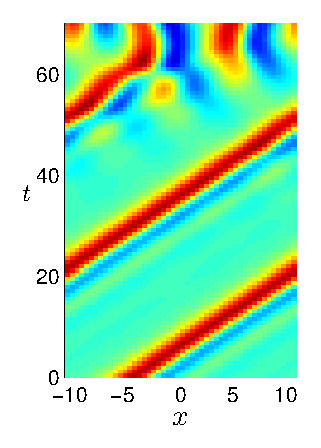
\includegraphics[width=0.3\textwidth, clip=true]{figs/ks22_TW1_orbit_c.eps}
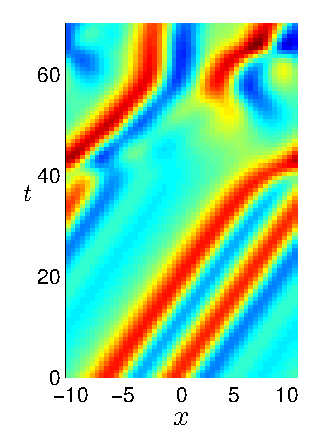
\includegraphics[width=0.3\textwidth, clip=true]{figs/ks22_TW2_orbit_c.eps}
\end{center}
\caption{
\Reqva : \REQV{+}{1} with velocity $\velRel = 0.737$ and \REQV{+}{2} with
velocity $\velRel = 0.350$.
The upper panels show the \reqva\ profiles.  The lower panels show
evolution of slightly perturbed \reqva\ and their decay into generic
turbulence. Each \reqv\ has a reflection symmetric partner related by
$u(x) \to -u(-x)$ travelling with velocity $-\velRel$.
} \label{f:ks22TW}
\end{figure}
%%%%%%%%%%%%%%%%%%%%%%%%%%%%%%%%%%%%%%%%%%%%%%%%%%%%%%%%%%%%%%%%%%

Consistent with the bifurcation diagram of \reffig{fig:ksBifDiag},
we find two pairs of \reqva\ \refeq{reqva} with velocities
$\velRel =\pm 0.73699$ and $\pm 0.34954$
which we label \REQV{\pm}{1} and \REQV{\pm}{2},
for `traveling waves.'
The profiles of the two \reqva\ and their time evolution
with eventual decay into the chaotic attractor are
shown in \reffig{f:ks22TW}.  The leading eigenvalues of
\REQV{\pm}{1} and \REQV{\pm}{2} are listed in \reftab{tab:Eksym}.

\refTab{tab:L22cminus} lists \eqv\ energy $E$,
the local Poincar\'e section return time $T$,
radially expanding Floquet multiplier $\ExpaEig_e$, and
the least contracting Floquet multiplier $\ExpaEig_c$
for all $L=22$ \eqva\ and \reqva.
The return time $T=2\pi/\eigIm[e]$ is given by the imaginary
part of the leading complex eigenvalue,
the expansion
multiplier per one turn of the most unstable spiral-out by
$\ExpaEig_e\approx\exp(\eigRe[e] T)$, and the contraction
rate along the slowest contracting stable eigendirection by
$\ExpaEig_c\approx\exp(\eigRe[c]T)$.
For \EQV{3} and \REQV{\pm}{2}, whose leading eigenvalues are
real, we use $T=1/\Lyap_1$ as the characteristic time scale.
While the complex eigenvalues set time scales of recurrences,
this time scale is useful for comparison of leading expanding
and the slowest contracting multiplier.
We learn that the shortest
`turn-over' time is $\approx 10-20$, and that if there exist
horseshoe sets of unstable \po s associated with
these \eqva,  they have unstable
multipliers of order of $\ExpaEig_e \sim 5-10$, and that
they are surprisingly thin in the folding direction, with
contracting multipliers of order of $10^{-2}$,
as also observed in \refref{lanCvit07}.

\begin{table}[ht]
    \caption{
    Properties of \eqva\ and \reqva\ determining
    the system dynamics in their vicinity.  $T$ is characteristic
    time scale of the dynamics, $\ExpaEig_e$ and $\ExpaEig_c$ are the
    leading expansion and contraction multipliers, and $E$ is the
    energy \refeq{ksEnergy}.
            }
\begin{center} \footnotesize
    \begin{tabular}{l|rrrr}
                 & $E$~~   & $T$~~  & $\ExpaEig_e$  & $\ExpaEig_c$  \\ \hline
 $\EQV{1}\ $     &\ 0.2609 &\ 18.81 &\ 11.70    &\ 0.01 \\ %Young ES had: \ExpaEig_e=4.79, \ExpaEig_c=0.04
 $\EQV{2}\ $     &\ 0.4382 &\ 26.35 &\ 39.00    &\ 0.11 \\ %Young ES had: \ExpaEig_e=5.99, \ExpaEig_c=0.03
 $\EQV{3}\ $     &\ 1.5876 &\ 10.72 &\ 2.72     &\ 0.01 \\ %ES had \ExpaEig_e=9.92
 $\REQV{\pm}{1}$ &\ 0.4649 &\  7.69 &\ 2.43     &\ 0.15 \\
 $\REQV{\pm}{2}$ &\ 0.6048 &\  2.97 &\ 2.72     &\ 0.97 \\ %PC entered 2.72 = e^1
    \end{tabular}
\end{center}
\label{tab:L22cminus}
\end{table}

\subsection{Unstable manifolds of \eqva\ and their heteroclinic
            connections}
\label{sec:unstMnflds}

As shown in \refTab{tab:Eksym},
the \EQV{1} \eqv\ has two unstable
planes within which the solutions are spiralling out (\ie, two
pairs of complex conjugate eigenvalues).  The \EQV{2} has one such plane,
while the \EQV{3} has two real positive eigenvalues, so the solutions are
moving radially away from the \eqv\ within the plane spanned
by the corresponding eigenvectors.  Since \EQV{1} has
a larger unstable subspace, it is expected to have much less influence on the
long time dynamics compared to \EQV{2} and \EQV{3}.

\begin{figure}[t]
\begin{center}
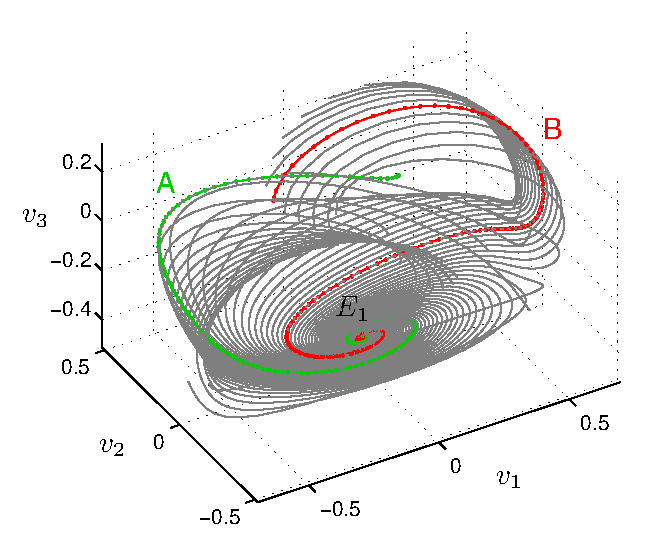
\includegraphics[width=0.5\textwidth, clip=true]{figs/ks22_E1_plane1_manifold_c.eps}
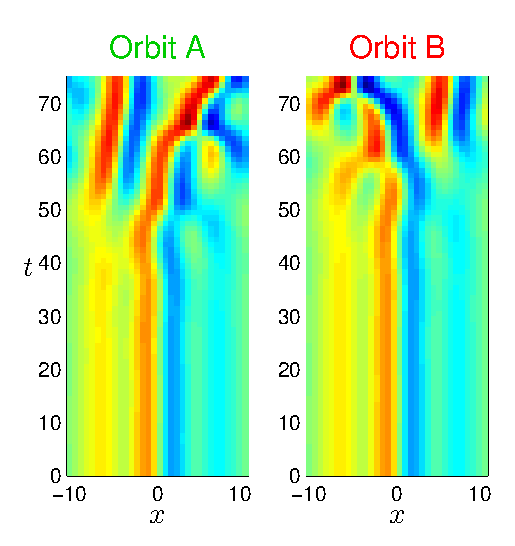
\includegraphics[width=0.4\textwidth, clip=true]{figs/ks22_E1_plane1_orbits_c.eps}
\end{center}
\caption{
The left panel shows the unstable
manifold of \eqv\ \EQV{1} starting within the plane
corresponding to the first pair of unstable eigenvalues. The
coordinate axes $v_1$, $v_2$, and $v_3$ are
projections onto three orthonormal vectors
$\mathbf{v}_1$, $\mathbf{v}_2$, and $\mathbf{v}_3$,
respectively,
constructed from vectors
$\Re \,\jEigvec{1}$, $\Im \,\jEigvec{1}$,
and $\Re \,\jEigvec{6}$
by Gram-Schmidt orthogonalization.
The right panel shows spatial representation of two orbits $A$ and $B$.
The change of color from blue to red indicates increasing values of
$u(x)$, as in the colorbar of \reffig{f:ks_largeL}.
}
\label{f:KS22E1man1}
\end{figure}

Many methods have been developed for visualization of stable
and unstable manifolds, see \refref{krauskopf_survey_2005}
for a survey. For high-dimensional contracting flows
visualization of stable manifolds is impossible, unless the
system can be restricted to an approximate  low-dimensional
inertial manifold, as, for example, in \refref{kev01ks}. The unstable
manifold visualization also becomes harder as its dimension
increases. Here we concentrate on visualizations of $1$-- and
$2$--dimensional unstable manifolds. Our visualization is
unsophisticated compared to the methods of
\refref{krauskopf_survey_2005}, yet sufficient for our
purposes since, as we shall see, the unstable manifolds we
study terminate in another equilibrium and thus there is no
need to track them for long times.


To construct an invariant manifold containing solutions
corresponding to the pair of unstable complex conjugate eigenvalues,
$\eigExp = \eigRe \pm i\eigIm$,
$\eigRe > 0$, we start with a set of
initial conditions near \eqv\ \EQV{k},
\beq
  a(0) = a_{{\EQV{k}}} + \epsilon\,\exp(\delta)\jEigvec{j}
\,,
\ee{linUnstMan}
where $\delta$ takes a set of values uniformly distributed in the
interval $[0,2\pi\eigRe/\eigIm]$, $\jEigvec{j}$ is a unit vector in the
unstable plane, and $\epsilon > 0$ is small.

\begin{figure}[t]
\begin{center}
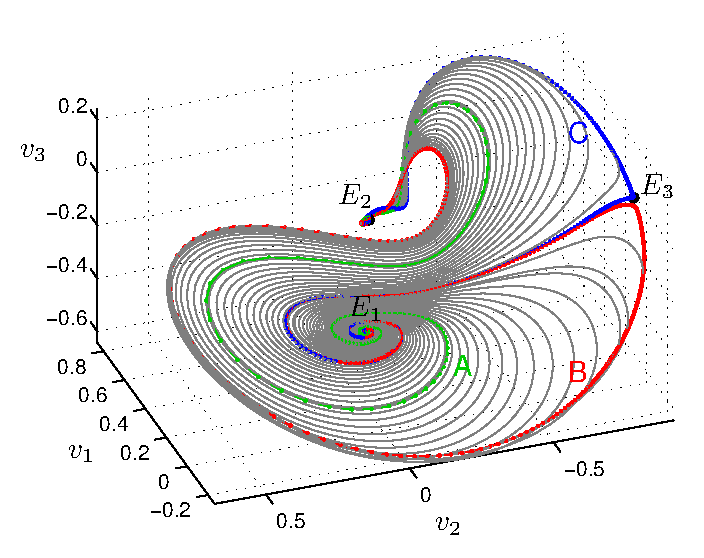
\includegraphics[width=0.48\textwidth, clip=true]{figs/ks22_E1_plane2_manifold_c.eps}
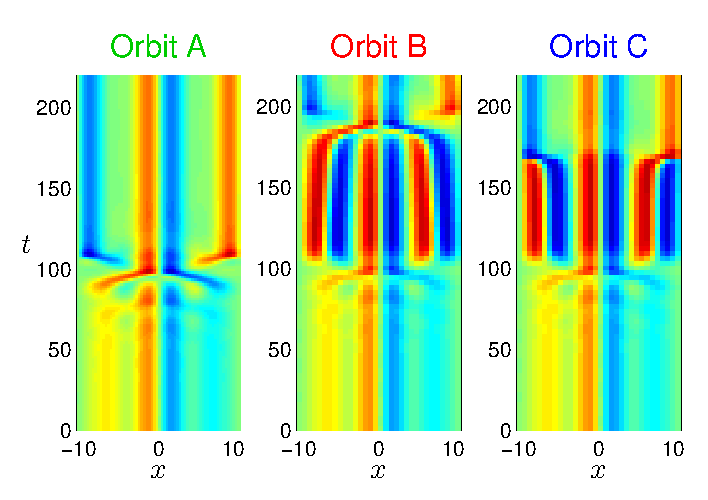
\includegraphics[width=0.48\textwidth, clip=true]{figs/ks22_E1_plane2_orbits_c.eps}
\end{center}
\caption{
The left panel shows the unstable
manifold of \eqv\ \EQV{1} starting within the plane
corresponding to the second pair of unstable eigenvalues. The
coordinate axes $v_1$, $v_2$, and $v_3$ are
projections onto three orthonormal vectors
$\mathbf{v}_1$, $\mathbf{v}_2$, and $\mathbf{v}_3$,
respectively, constructed from vectors
\Re\, $\jEigvec{3}$, \Im\, $\jEigvec{3}$, and \Re\, $\jEigvec{6}$
by Gram-Schmidt orthogonalization.
The right panel shows spatial representation of three orbits. Orbits
$B$ and $C$ pass close to the \eqv\ \EQV{3}.
   }
\label{f:KS22E1man2}
\end{figure}

The manifold starting within the first unstable plane of \EQV{1}, with
eigenvalues $0.1308\pm i\,0.3341$, is shown in
\reffig{f:KS22E1man1}. It appears to fall directly into the
chaotic attractor.  The behavior of the manifold starting within
the second unstable plane of \EQV{1}, eigenvalues $0.0824\pm i \, 0.3402$, is
remarkably different: as can be seen in \reffig{f:KS22E1man2},
almost all orbits within the manifold converge to the \eqv\ \EQV{2}.  The
manifold also contains a heteroclinic connection from \EQV{1} to \EQV{3},
and is bordered by the $\eigExp[1]$-eigendirection
unstable manifold of \EQV{3}.

\begin{figure}[ht]
\begin{center}
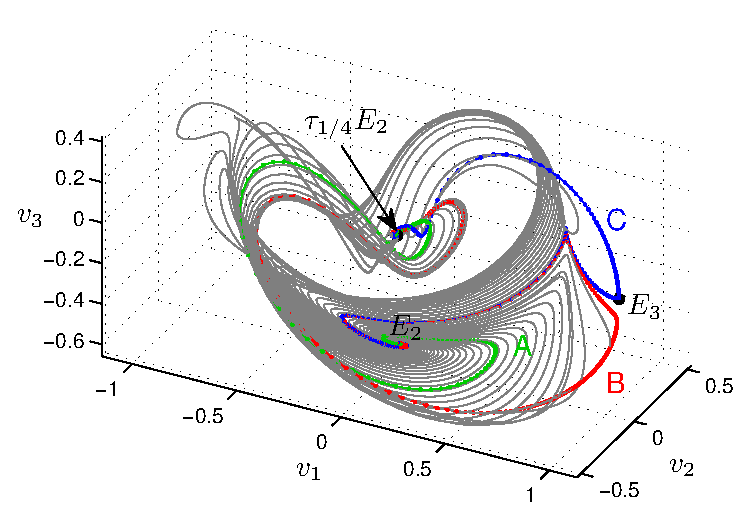
\includegraphics[width=0.48\textwidth, clip=true]{figs/ks22_E2_manifold_c.eps}
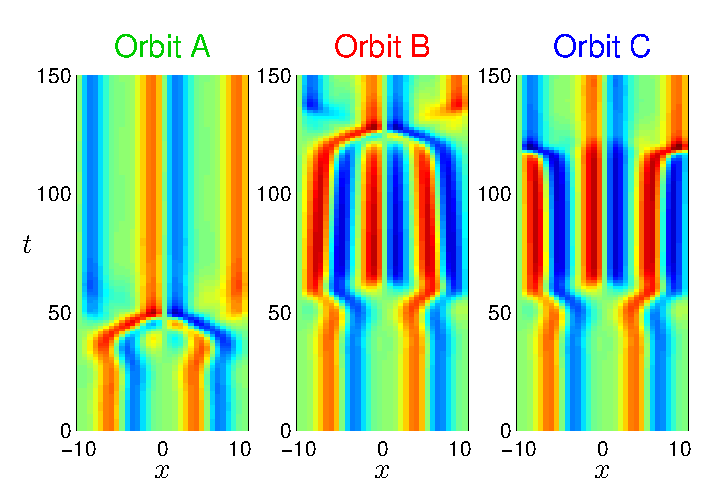
\includegraphics[width=0.48\textwidth, clip=true]{figs/ks22_E2_orbits_c.eps}
\end{center}
\caption{
The left panel shows the two-dimensional
unstable manifold of \eqv\ \EQV{2}. The coordinate axes
$v_1$, $v_2$, and $v_3$ are
projections onto three orthonormal vectors
$\mathbf{v}_1$, $\mathbf{v}_2$, and $\mathbf{v}_3$,
respectively, constructed from vectors
\Re\, $\jEigvec{1}$, \Im\, $\jEigvec{1}$, and \Re\, $\jEigvec{7}$
by Gram-Schmidt orthogonalization.
The right panel shows spatial representation of three orbits. Orbits
$B$ and $C$ pass close to the \eqv\ \EQV{3}. See
\reffig{f:KS22Manifold} for a different visualization.
       }
\label{f:KS22E2man}
\end{figure}


%%%%%%%%%%%%%%%%%%%%%%%%%%%%%%%%%%%%%%%%%%%%%%%%%%%%%%%%%%%%%%%%
\begin{figure}[t]
\begin{center}
%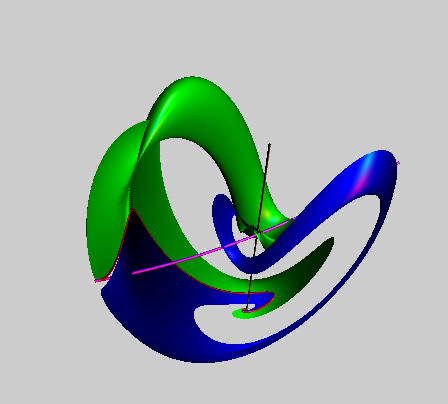
\includegraphics[width=0.6\textwidth, clip=true]{figs/ks22manifold.ps}
(\textit{a}) 
\includegraphics[width=0.4\textwidth, clip=true]{figs/ks22manifold1.eps}
(\textit{b}) 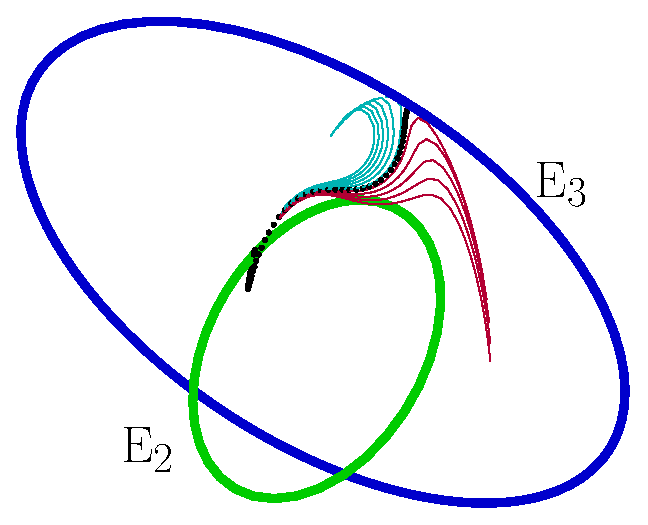
\includegraphics[width=0.4\textwidth, clip=true]{figs/ks22E2-E3hetero.eps}
\end{center}
\caption{
(a) (blue/green) The unstable manifold of \EQV{2}~\eqv, projection
	in the coordinate axes of \reffig{f:KS22E2man}.
    (black line) The circle of \EQV{2}~\eqva\
related by the translation invariance.
(purple line) The circle  of \EQV{3}~\eqva.
(red) The heteroclinic connection
from the \EQV{2}~\eqv\ to the \EQV{3}~\eqv\ splits
the manifold into two parts,
colored (blue) and (green).
(b) \EQV{2}~\eqv\ to \EQV{3}~\eqv\ heteroclinic
connection, $(\Re\, \jEigvec{2}, \Re\, \jEigvec{3}, ( \Im\, \jEigvec{2} + \Im\, \jEigvec{3})/\sqrt{2})$ projection. 
Here we omit the unstable manifold of \EQV{2},
keeping only a few neighboring trajectories in order to indicate
the unstable manifold of \EQV{3}. The \EQV{2} and \EQV{3}
families of \eqva\ arising from the continuous translational
symmetry of KS on a periodic domain are indicated by the two circles.
        }
\label{f:KS22Manifold}
\end{figure}
%%%%%%%%%%%%%%%%%%%%%%%%%%%%%%%%%%%%%%%%%%%%%%%%%%%%%%%%%%%%%%%%%%

The two-dimensional unstable manifold of \EQV{2} is shown in
\reffig{f:KS22E2man}.  All orbits within the manifold, except
for the heteroclinic connections from \EQV{2} to \EQV{3}, converge
to \EQV{2} shifted by $L/4$,
so this manifold, minus the heteroclinic connections, can be viewed as
a homoclinic connection.  %It also contains a pair of heteroclinic connections from
%\EQV{2} to \EQV{3}.

The \eqv\ \EQV{3} has a pair of real unstable eigenvalues
equal to each other.  Therefore, within the plane spanned by the
corresponding eigenvectors, the orbits move radially away from
the \eqv.  In order to trace out the unstable manifold,
we start with a set of initial conditions within the unstable plane
\beq
 a(0) = a_{{\EQV{3}}} + \epsilon(\mathbf{v}_1 \cos \phi + \mathbf{v}_2 \sin \phi)\,,
  \quad\phi\in[0,2\pi]\,,
\label{unsManSeed}
\eeq
where $\mathbf{v}_1$ and $\mathbf{v}_2$ are orthonormal vectors within the
plane spanned by the two unstable eigenvectors.
%, seeded as in \refeq{linUnstMan}.
  The unstable manifold
of \EQV{3} is shown in \reffig{f:KS22E3man}.  The 3-fold symmetry of
the manifold is related to the symmetry of \EQV{3} with respect to
translation by $L/3$.  The manifold contains heteroclinic orbits
connecting \EQV{3} to three different points of the circle of {\eqva}
\EQV{2} translated set of solutions. Note also that the segments of orbits $B$ and $C$
between \EQV{3} and \EQV{2} in \reffigs{f:KS22E1man2}{f:KS22E2man}
represent the same heteroclinic connections as orbits $B$ and $C$ in
\reffig{f:KS22E3man}.

%%%%%%%%%%%%%%%%%%%%%%%%%%%%%%%%%%%%%%%%%%%%%%%%%%%%%%%%%%%%%%%%
\begin{figure}[t]
\begin{center}
\includegraphics[width=0.45\textwidth, clip=true]{figs/ks22_E3_manifold.eps}
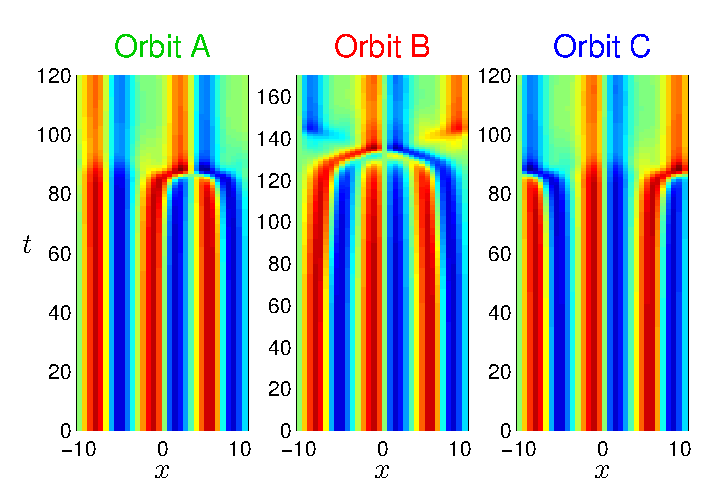
\includegraphics[width=0.5\textwidth, clip=true]{figs/ks22_E3_orbits_c.eps}
\end{center}
\caption{
The left panel shows the two-dimensional
unstable manifold of \eqv\ \EQV{3}. The coordinate axes
$v_1$, $v_2$, and $v_3$ are
projections onto three orthonormal vectors
$\mathbf{v}_1$, $\mathbf{v}_2$, and $\mathbf{v}_3$,
respectively, constructed from vectors
$\jEigvec{1}$, $\jEigvec{2}$, and $\jEigvec{4}$ by Gram-Schmidt orthogonalization.
The black line shows a family of \EQV{2}~\eqva\ related by translational
symmetry. The right panel shows spatial representation of
three orbits. Orbits $B$ and $C$ are two different heteroclinic orbits
connecting \EQV{3} to the same point on the \EQV{2} line.
        }
\label{f:KS22E3man}
\end{figure}
%%%%%%%%%%%%%%%%%%%%%%%%%%%%%%%%%%%%%%%%%%%%%%%%%%%%%%%%%%%%%%%%

Heteroclinic connections are non-generic for high-dimensional
systems, but can be robust in systems with continuous
symmetry, see \refref{KrupaRobHetCyc97} for a review.
Armbruster \etal\rf{AGHks89} study a fourth order truncation
of KS dynamics on the center-unstable manifold of $\EQV{2}$
close to a bifurcation off the constant $u(x,t)=0$ solution
and prove existence of a heteroclinic connection, see also
\refref{AGHO288}. Kevrekidis \etal\rf{KNSks90} study the
dynamics numerically and establish the existence of a robust
heteroclinic connection for a range of parameters close to
the onset of the 2-cell branch in terms of the symmetry and a
flow invariant subspace. We adopt their arguments to explain
the new heteroclinic connections
shown in \reffig{f:KS22hetero} that
we have found for $L=22$.
For our system size there are exactly two representatives of
the $\EQV{2}$ family that lie in the intersection of $\bbU^+$
and $\bbU^{(1)}$ related to each other by an $L/4$ shift.
Denote them by $\EQV{2}$ and $\Shift_{1/4}\EQV{2}$
respectively. The unstable eigenplane of $\EQV{2}$ lies on
$\bbU^+$ while that of $\Shift_{1/4}\EQV{2}$ lies on
$\bbU^{(1)}$, \cf\ \reftab{tab:Eksym}. The $\EQV{3}$ family
members that live in $\bbU^+$ have one of their unstable
eigenvectors (the one related to the heteroclinic connection
to $\EQV{2}$ family)  on $\bbU^+$, while the other does not
lie on symmetry-invariant subspace. Similarly, for the
$\EQV{1}$ family we observe that the equilibria in $\bbU^+$
have an unstable plane on $\bbU^+$ (again related to the
heteroclinic connection) and a second one with no symmetry.
Thus $\Shift_{1/4}\EQV{2}$ appears as a sink on $\bbU^+$,
while all other equilibria appear as sources. This explains
the heteroclinic connections from $\EQV{1}\,,\EQV{2}$ and
$\EQV{3}$ to $\Shift_{1/4}\EQV{2}$. Observing that
$\Shift_{1/4} \bbU^+= \bbU^{(1)}$ and taking into account
\reftab{tab:Eksym} we understand that within $\bbU^{(1)}$ we
have connections from $\Shift_{1/4}\EQV{2}$ (and members of
$\EQV{1}$ and $\EQV{3}$ families) to $\EQV{2}$ and the
formation of a heteroclinic loop. Due to the translational
invariance of KS there is a heteroclinic loop for any two
points of the $\EQV{2}$ family related by an $\Shift_{1/4}$-shift.

%%%%%%%%%%%%%%%%%%%%%%%%%%%%%%%%%%%%%%%%%%%%%%%%%%%%%%%%%%%%%%%%
\begin{figure}[t]
\begin{center}
        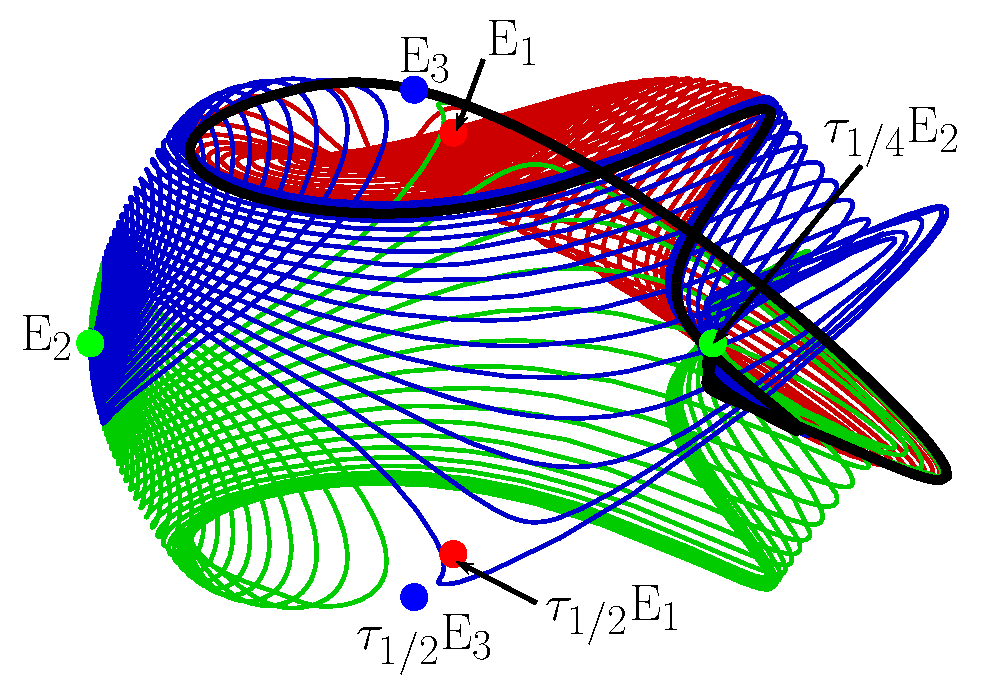
\includegraphics[width=0.6\textwidth, clip=true]{figs/KS22hetero.eps}
\end{center}
\caption{ Heteroclinic connections on $\bbU^+$:
 (red) The unstable manifold of \EQV{1}~\eqv.
 (blue/green) The unstable manifold of \EQV{2}~\eqv.
 (black) Heteroclinic connections from \EQV{3}~\eqv\ to $\Shift_{1/4}$\EQV{2}~\eqv,
 where $ \Shift_{1/m}u(x)=u(x+L/m)$ is a rational shift \refeq{eq:shiftFour}.
 Projection from $128$ dimensions onto the plane given by the vectors
 $a_{\EQV{2}}-a_{\Shift_{1/4}\EQV{2}}$ and $a_{\EQV{3}}-a_{\Shift_{1/2}\EQV{3}}$.}
\label{f:KS22hetero}
\end{figure}
%%%%%%%%%%%%%%%%%%%%%%%%%%%%%%%%%%%%%%%%%%%%%%%%%%%%%%%%%%%%%%%%%%



\section{\Rpo s for $L=22$}
\label{sec:rpos}

The \rpo s satisfy the condition \refeq{KSrpos}
$u(x+\shift_p,\period{p}) = u(x,0)$,
where $\period{p}$ is the period and $\shift_p$ the phase shift.
We have limited our search to orbits with $\period{p} < 200$ and found
over 30\,000 \rpo s with $\shift_p > 0$.  The details of the algorithm
used and the search strategy employed are given in
\refappe{sec:lmderRLD}.
Each \rpo\ with phase shift
$\shift_p > 0$ has a reflection symmetric partner
$u_p(x) \to -u_p(-x)$ with phase shift $-\shift_p$.

The small period \rpo s outline the coarse structure of the chaotic
attractor, while the longer period \rpo s resolve the finer details
of the dynamics.
The first four orbits with the shortest periods we have found are
shown in \reffig{f:ks22rpos}\,(\textit{a-d}).  The shortest \rpo\ with
$\period{p} = 16.4$ is also the most unstable, with one positive
Floquet exponent equal 0.328.  The other short orbits are less
unstable, with the largest Floquet exponent in the range
0.018 -- 0.073, typical of the long time attractor average.

%%%%%%%%%%%%%%%%%%%%%%%%%%%%%%%%%%%%%%%%%%%%%%%%%%%%%%%%%%%%%%%%
\begin{figure}[t]
\begin{center}
\begin{tabular}{cccccc} (\textit{a}) & (\textit{c}) & (\textit{e}) &
                        (\textit{g}) & (\textit{i}) & (\textit{k})\\
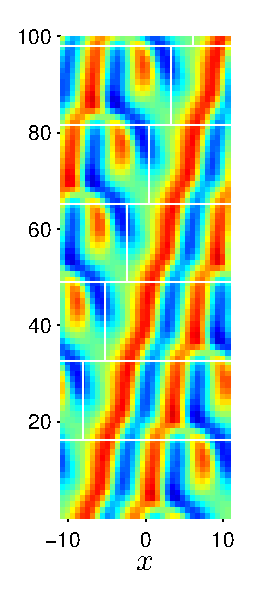
\includegraphics[width=0.15\textwidth, clip=true]{figs/ks22rpo016.3-02.86.eps}\hspace{-3ex} &
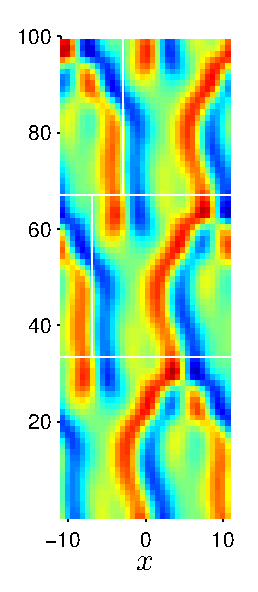
\includegraphics[width=0.15\textwidth, clip=true]{figs/ks22rpo033.5-04.04.eps}\hspace{-3ex} &
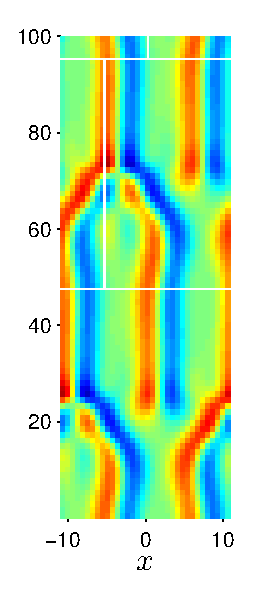
\includegraphics[width=0.15\textwidth, clip=true]{figs/ks22rpo047.6-05.68.eps}\hspace{-3ex} &
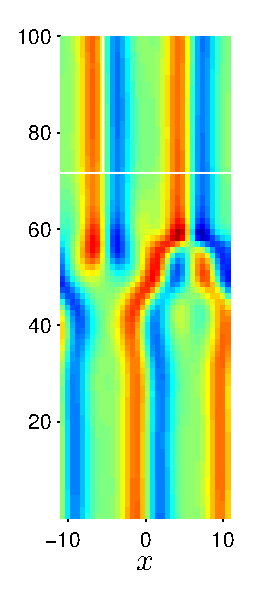
\includegraphics[width=0.15\textwidth, clip=true]{figs/ks22rpo071.7-05.50.eps}\hspace{-3ex} &
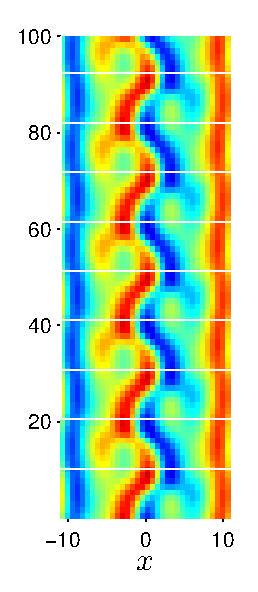
\includegraphics[width=0.15\textwidth, clip=true]{figs/ks22rpo020.5-00.00.eps}\hspace{-3ex} &
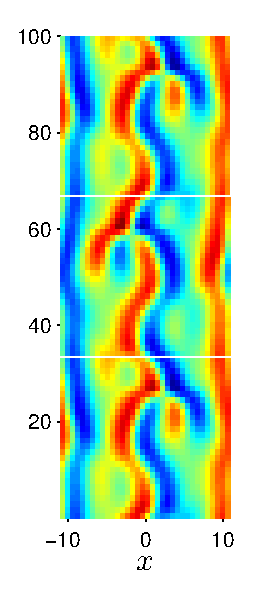
\includegraphics[width=0.15\textwidth, clip=true]{figs/ks22rpo066.8-00.00.eps}\\
(\textit{b}) & (\textit{d}) & (\textit{f}) &
(\textit{h}) & (\textit{j}) & (\textit{l})\\
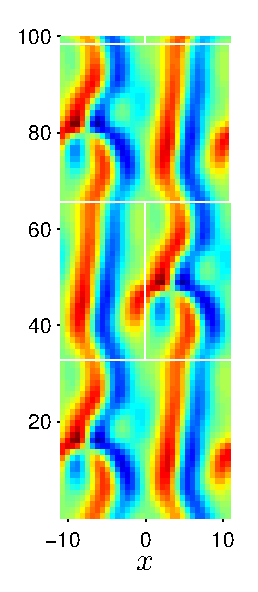
\includegraphics[width=0.15\textwidth, clip=true]{figs/ks22rpo032.8-10.96.eps}\hspace{-3ex} &
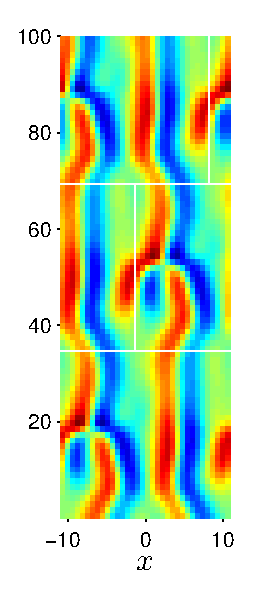
\includegraphics[width=0.15\textwidth, clip=true]{figs/ks22rpo034.6-09.60.eps}\hspace{-3ex} &
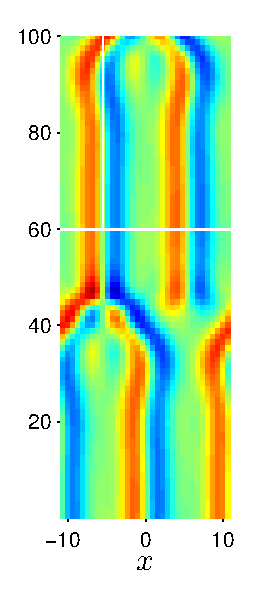
\includegraphics[width=0.15\textwidth, clip=true]{figs/ks22rpo059.9-05.44.eps}\hspace{-3ex} &
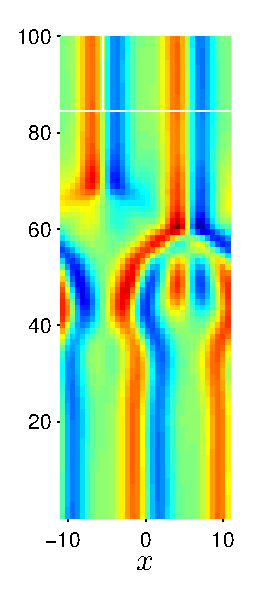
\includegraphics[width=0.15\textwidth, clip=true]{figs/ks22rpo084.4-05.51.eps}\hspace{-3ex} &
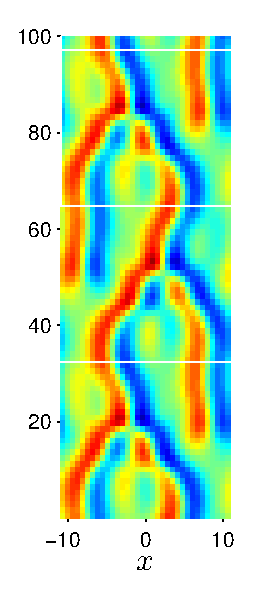
\includegraphics[width=0.15\textwidth, clip=true]{figs/ks22rpo064.7-00.00.eps}\hspace{-3ex} &
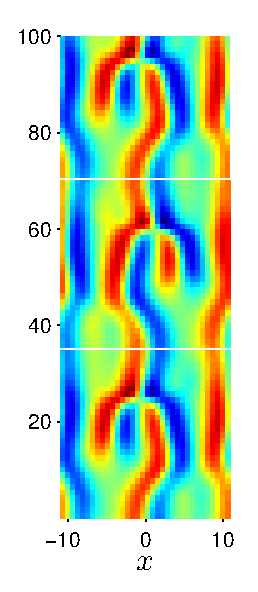
\includegraphics[width=0.15\textwidth, clip=true]{figs/ks22rpo070.3-00.00.eps}
\end{tabular}
\end{center}
\caption{Selected relative periodic and
pre-periodic
orbits of KS flow with $L = 22$:
(a) $\period{p} = 16.3$, $\shift_p = 2.86$;
(b) $\period{p} = 32.8$, $\shift_p = 10.96$;
(c) $\period{p} = 33.5$, $\shift_p = 4.04$;
(d) $\period{p} = 34.6$, $\shift_p = 9.60$;
(e) $\period{p} = 47.6$, $\shift_p = 5.68$;
(f) $\period{p} = 59.9$, $\shift_p = 5.44$;
(g) $\period{p} = 71.7$, $\shift_p = 5.503$;
(h) $\period{p} = 84.4$, $\shift_p = 5.513$;
(i) $\period{p} = 10.3$;
(j) $\period{p} = 32.4$;
(k) $\period{p} = 33.4$;
(l) $\period{p} = 35.2$.
Horizontal and vertical white lines indicate periodicity and phase
shift of the orbits, respectively.
}\label{f:ks22rpos}
\end{figure}
%%%%%%%%%%%%%%%%%%%%%%%%%%%%%%%%%%%%%%%%%%%%%%%%%%%%%%%%%%%%%%%%


We have found \rpo s which stay
close to the unstable manifold of \EQV{2}.
As is illustrated in \reffig{f:ks22rpos}\,(\textit{e-h}), all such orbits have
shift $\shift_p \approx L/4$, similar to the shift of orbits within
the unstable manifold of \EQV{2}, which start at \EQV{2} and
converge to $\Shift_{1/4}$\EQV{2} (see \reffig{f:KS22E2man}). This
confirms that the `cage' of unstable manifolds of equilibria plays
an important role in organizing the chaotic dynamics of the KS
equation.


\section{Pre-periodic orbits} \label{ssec:po}

As discussed in \refSect{sec:KSePO}, a \rpo\ will be
periodic, \ie, $\shift_p = 0$, if it either {\bf (a)} lives
within the $\bbU^+$ antisymmetric subspace, $-u(-x,0) =
u(x,0)$, or {\bf (b)} returns to its reflection
or its discrete rotation after a period:
$u(x,t+\period{p})=\gamma u(x,t)$, $\gamma^m=e$,
and is thus periodic with period $m\period{p}$.
The dynamics of KS flow in the antisymmetric subspace and \po
s with symmetry {\bf (a)} have been investigated
previously\rf{Christiansen97,LanThesis,lanCvit07}.
%     \PC{this seems to have vanished, but I remember citing the system
%     sizes: Vaggelis, if there is time please complete:
%     ``at system sizes $L=...$ and $L=...$.''}
The KS flow does not have any periodic orbits of this type
for $L = 22$.

Using the algorithm and strategy described in
\refappe{sec:lmderRLD}, we have found over 30\,000
pre-periodic orbits with $\period{p} < 200$ which possess the
symmetry of type {\bf (b)} with $\gamma=\Refl\in D_1$.
Some of the shortest such orbits we have found are shown in
\reffig{f:ks22rpos}\,(\textit{i-l}). Several were found as
repeats of pre-periodic orbits during searches for \rpo s
with non-zero shifts, while most have been found as solutions
of the pre-periodic orbit condition \refeq{KSpos} with
reflection, which takes form
\beq
 -\mathbf{g}(-\shift)a^\ast(\period{p}) = a(0)\,.
\label{KSposFour}
\eeq
in the Fourier space representation
(compare this to the condition \refeq{eq:system} for \rpo s).


\section{Energy transfer rates  for $L=22$}
\label{sec:energyL22}


%%%%%%%%%%%%%%%%%%%%%%%%%%%%%%%%%%%%%%%%%%%%%%%%%%%%%%%%%%%%%%%%
\begin{figure}[t]
\begin{center}
 \begin{tabular}{cc}
        ~~~~~~~~(\textit{a})                        &   ~~~~~~~~(\textit{b}) \\
    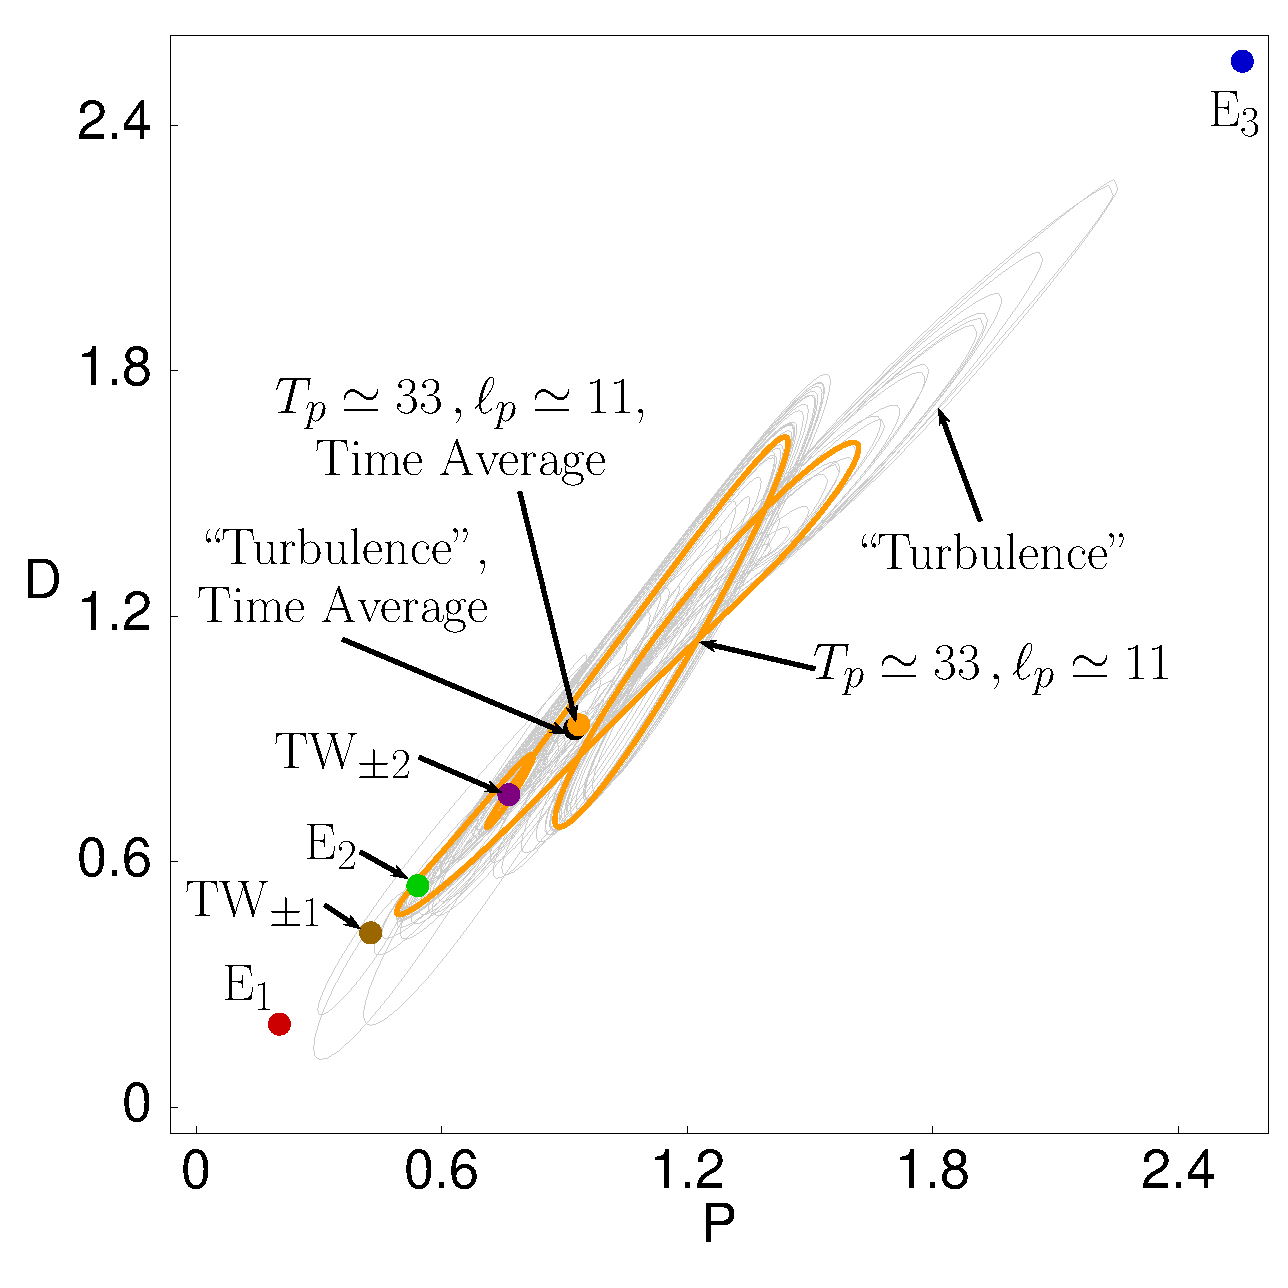
\includegraphics[width=0.46\textwidth, clip=true]{figs/energyBalance_pst.eps}  & 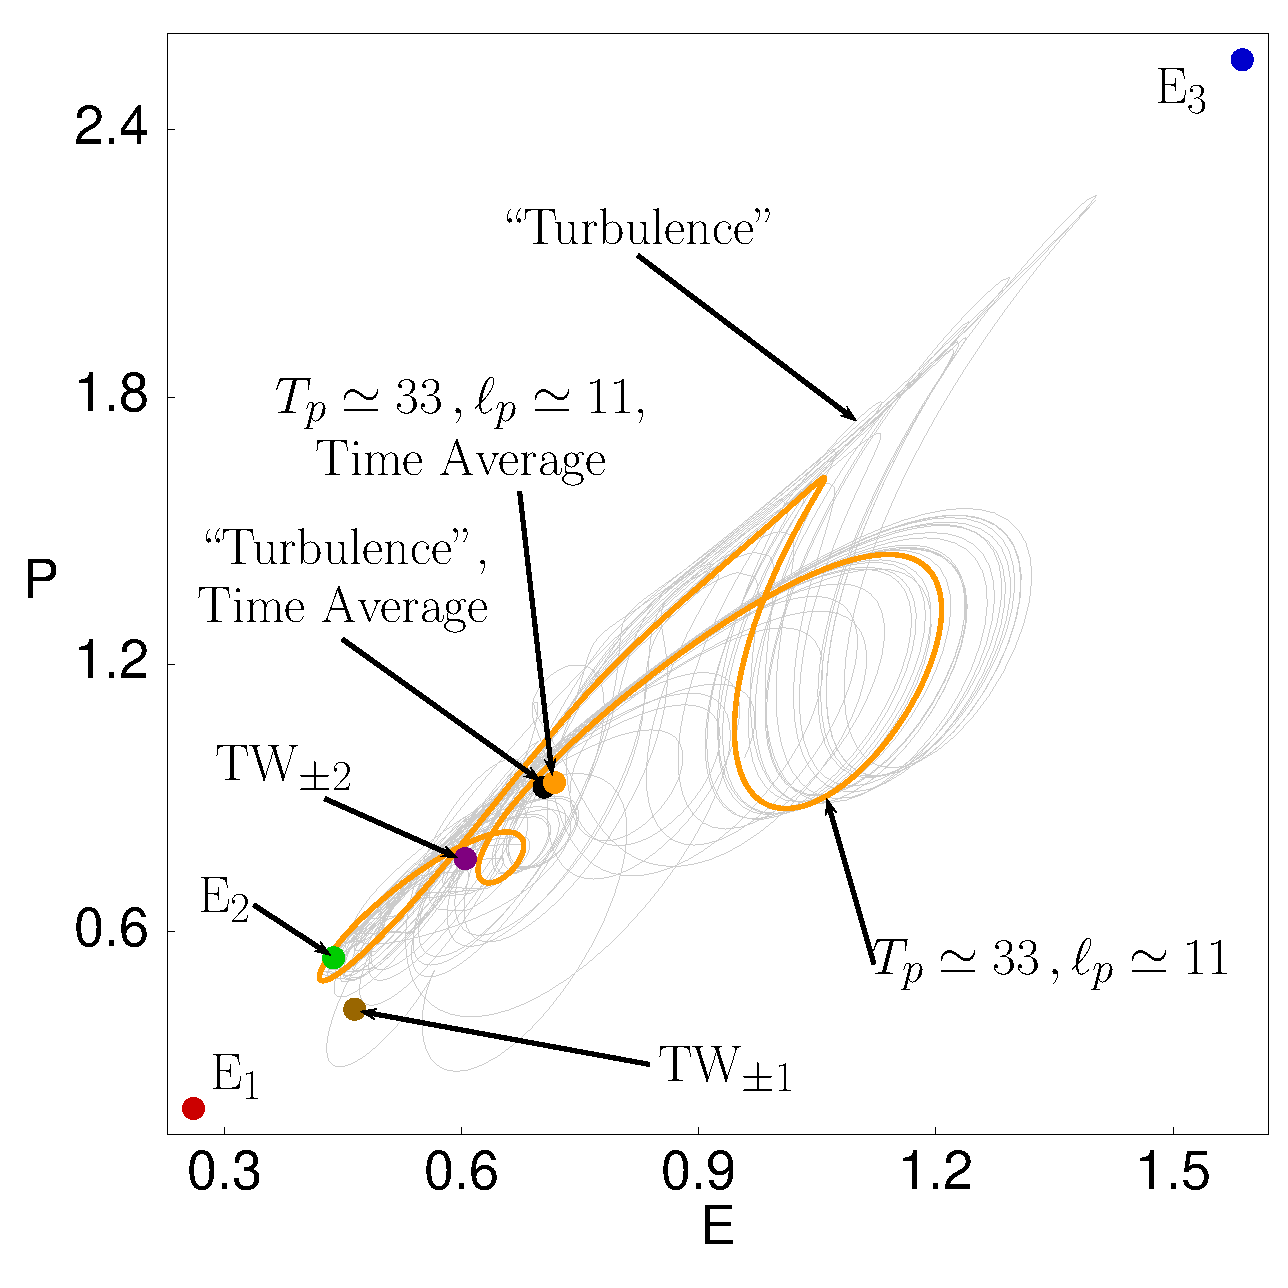
\includegraphics[width=0.46\textwidth, clip=true]{figs/equivaEP_pst.eps}

  \end{tabular}
\end{center}
\caption{
(a) Power input $P$ {\em vs.}
dissipation rate $D$
(b) energy $E$  {\em vs.}
power input $P$,   for several  \eqva\ and \reqva,
a \rpo, and a typical `turbulent' long-time trajectory.
Projections of the heteroclinic connections are
given in \reffig{f:drivedragConn}.
System size $L=22$.
        }
\label{f:drivedrag}
\end{figure}
%%%%%%%%%%%%%%%%%%%%%%%%%%%%%%%%%%%%%%%%%%%%%%%%%%%%%%%%%%%%%%%%%%

%%%%%%%%%%%%%%%%%%%%%%%%%%%%%%%%%%%%%%%%%%%%%%%%%%%%%%%%%%%%%%%%
\begin{figure}[t]
\begin{center}
 \begin{tabular}{cc}
        ~~~~~~~~(\textit{a})                        &   ~~~~~~~~(\textit{b}) \\
    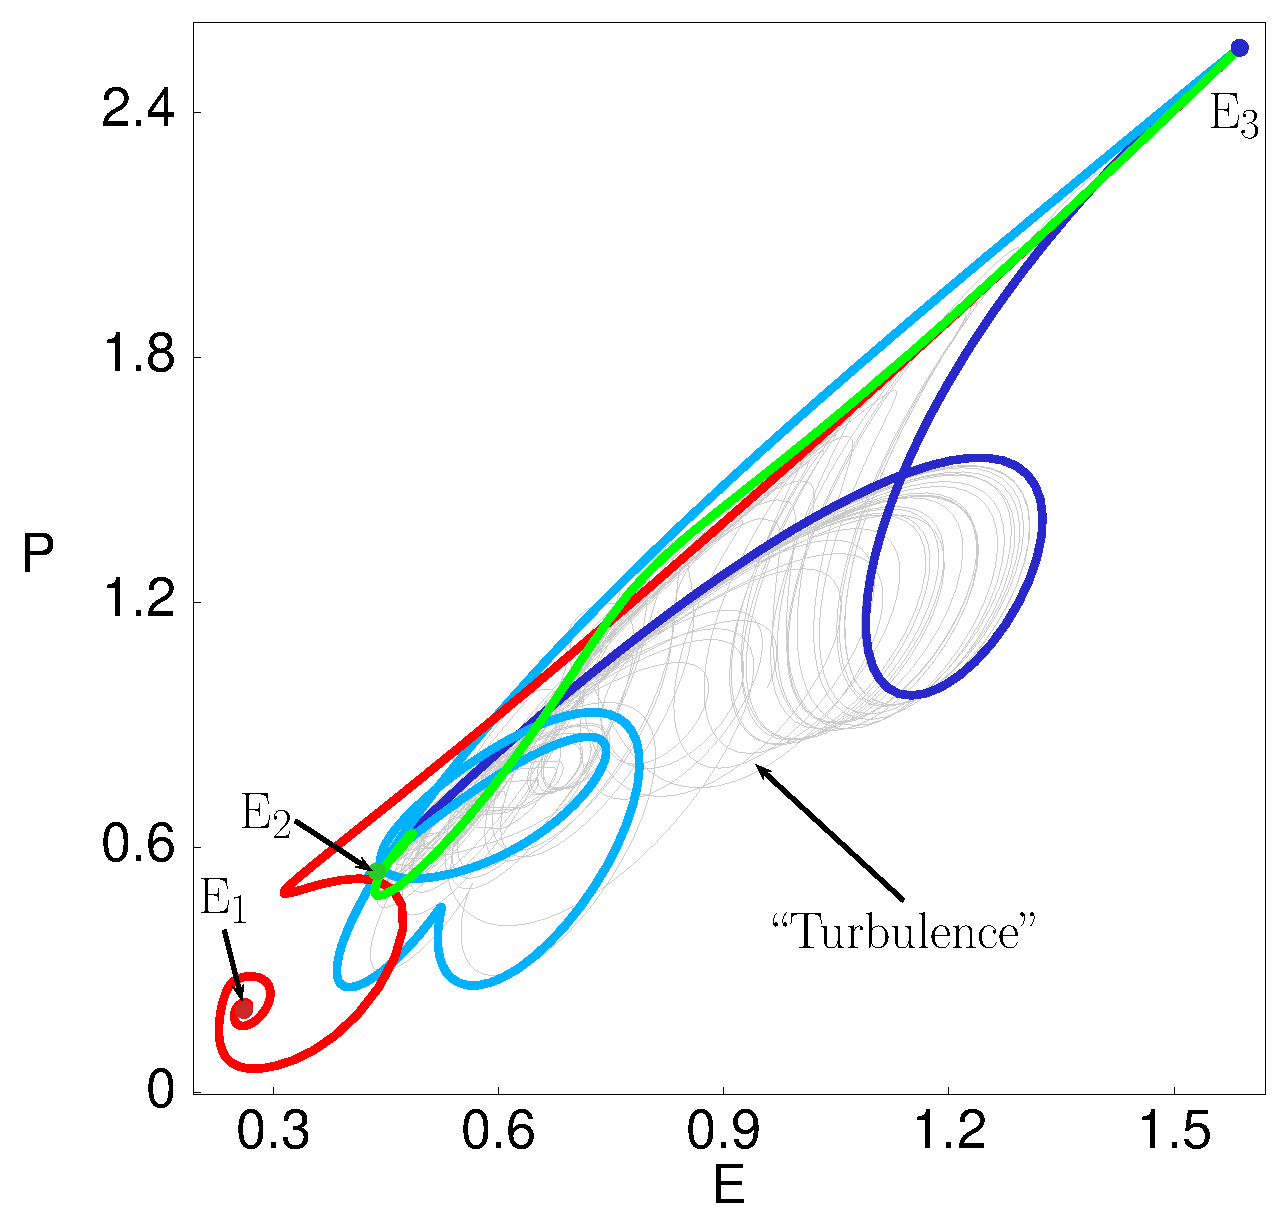
\includegraphics[width=0.46\textwidth, clip=true]{figs/connEP_pst.eps}     & 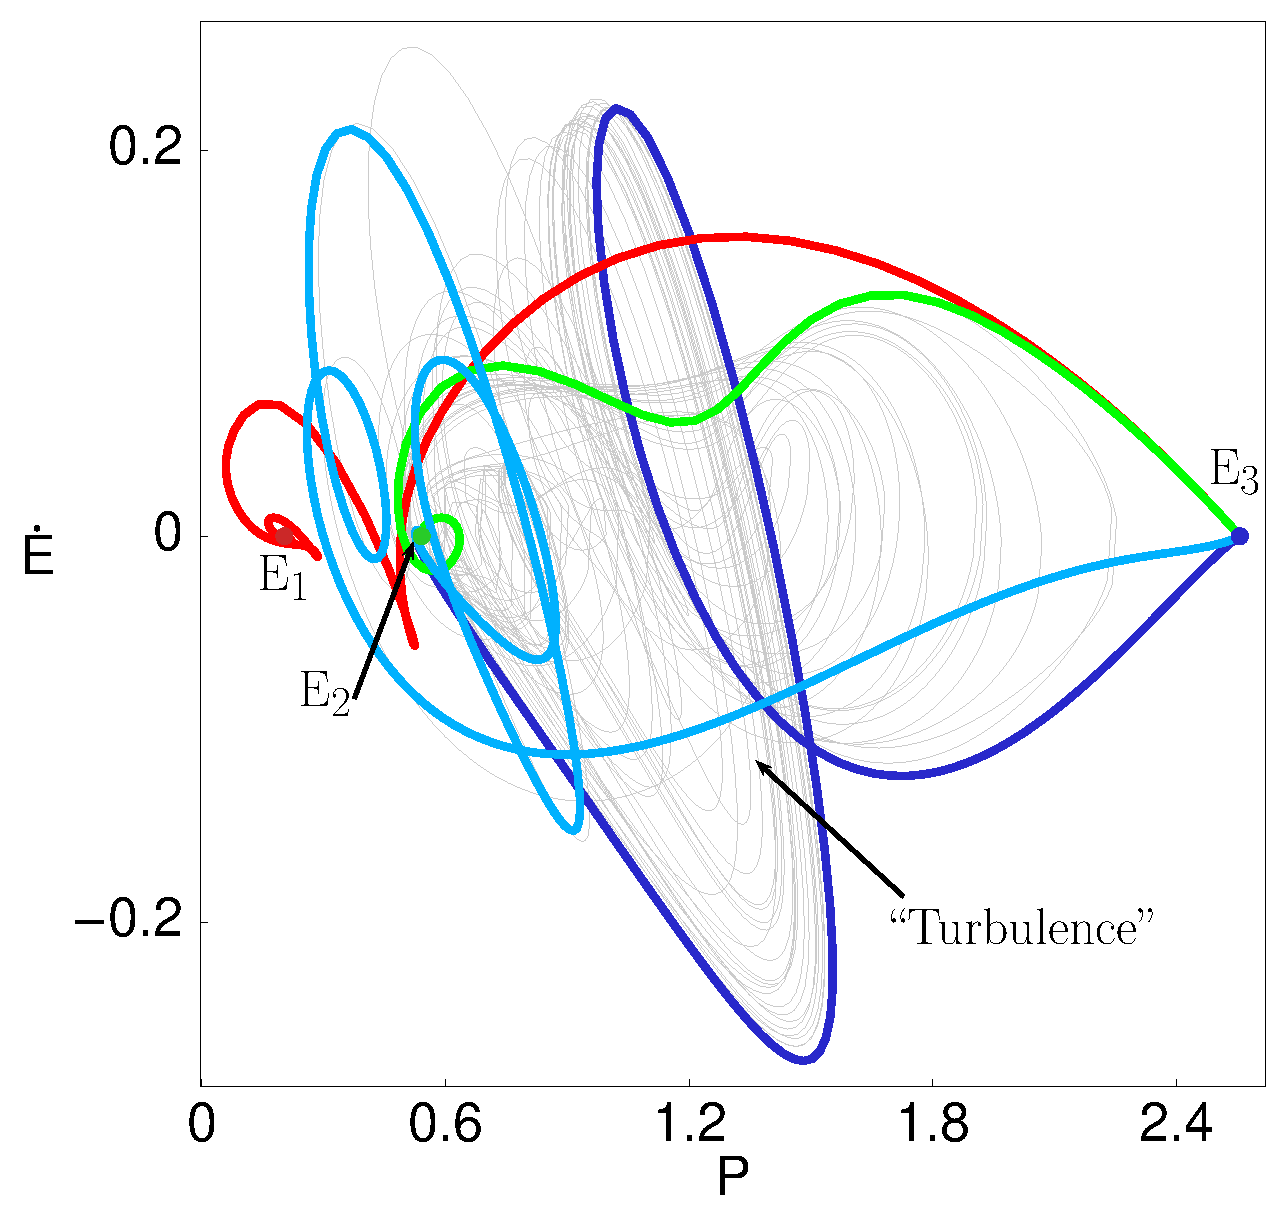
\includegraphics[width=0.46\textwidth, clip=true]{figs/connPEdot_pst.eps}
 \end{tabular}
\end{center}
\caption{
Two projections of the $(E,P,\dot{E})$ representation of the flow.
\EQV{1} (red), \EQV{2} (green), \EQV{3} (blue),
heteroclinic connections from \EQV{2} to $\EQV{3}$ (green),
from $\EQV{1}$ to \EQV{3} (red)
and from \EQV{3} to $\EQV{2}$ (shades of blue), superimposed over
a generic long-time `turbulent' trajectory (grey).
(a) As in \reffig{f:drivedragConn}\,(\textit{b}),
with labels omitted for clarity.
(b) A plot of  $\dot{\expctE} = P - D$ yields a clearer
visualization than \reffig{f:drivedragConn}\,(\textit{a}).
System size $L=22$.
        }
\label{f:drivedragConn}
\end{figure}
%%%%%%%%%%%%%%%%%%%%%%%%%%%%%%%%%%%%%%%%%%%%%%%%%%%%%%%%%%%%%%%%%%

In \reffig{f:drivedrag} we plot \refeq{EnRate}, the time-dependent
$\dot{\expctE}$ in the power input $P$ {\em vs.}
dissipation rate $D$ plane, for $L=22$ \eqva\ and \reqva,
a selected \rpo, and for a typical `turbulent' long-time
trajectory.

Projections from the $\infty$-dimensional \statesp\ onto the 3-dimensional
$(E,P,D)$ representation of the flow, such as
\reffigs{f:drivedrag}{f:drivedragConn}, can be misleading.
The most one can say is that if points are clearly separated in an
$(E,P,D)$ plot (for example, in \reffig{f:drivedrag}
$\EQV{1}$ \eqv\ is outside the recurrent set), they are also separated
in the full \statesp.  Converse is not true -- states of
very different topology can have similar energies.

An example is
the \rpo\ $(\period{p},\shift_p) = (32.8,10.96)$
(see \reffig{f:ks22rpos}\,(\textit{b})) which is the least
unstable short \rpo\ we have detected in this system. It appears to be
well embedded within the turbulent flow. The mean power $\timeAver{P_p}$ evaluated
as in \refeq{poE}, see \reffig{f:drivedrag},
is numerically quite close to the long-time
turbulent time average $\timeAver{P}$.
Similarly close prediction of mean dissipation rate in the
\pCf\ from a single-period \po\ computed by
Kawahara and Kida\rf{KawKida01} has lead to
optimistic hopes that `turbulence' is different from
low-dimensional chaos, insofar that the determination of one special
\po\ could yield all long-time averages.
Regrettably, not true -- as always, here too one needs a hierarchy
of \po s of increasing length to obtain accurate
predictions\rf{DasBuch}.

%%%%%%%%%%%%%%%%%%%%%%%%%%%%%%%%%%%%%%%%%%%%%%%%%%%%%%%%%%%%%%%%
\begin{figure}[t]
\begin{center}
(\textit{a})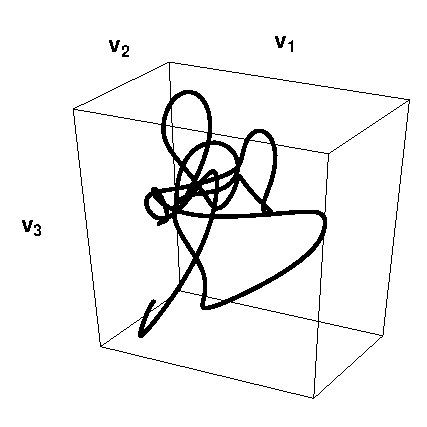
\includegraphics[width=0.46\textwidth, clip=true]{figs/ks22rpo033.50_04.045E2.eps}
(\textit{b})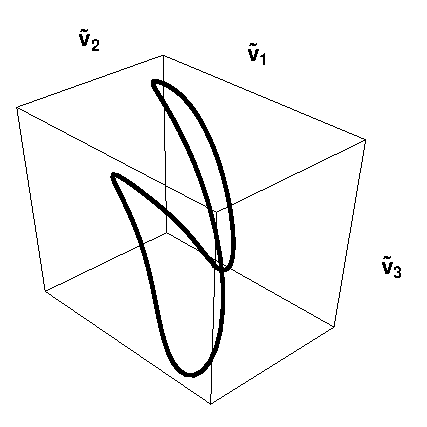
\includegraphics[width=0.46\textwidth, clip=true]{figs/ks22rpo033.50_04.045E2CM.eps}
\\
\end{center}
\caption{
 The
\rpo\ with $(\period{p},\shift_p) =(33.5,4.04)$
from \reffig{f:ks22rpos}\,(\textit{c})
which appears well embedded within the turbulent flow:
 (a) A stationary \statesp\ projection,
  traced for four periods $\period{p}$. The coordinate axes
$v_1$, $v_2$, and $v_3$ are those of \reffig{f:KS22E2man};
 (b) In the co-moving mean velocity frame.
%PC dropped this: traced for one period $\period{p}$.
        } \label{f:MeanVelocityFrame}
\end{figure}
%%%%%%%%%%%%%%%%%%%%%%%%%%%%%%%%%%%%%%%%%%%%%%%%%%%%%%%%%%%%%%%%%%

For any given \rpo\ a convenient visualization is
offered by the {\em mean velocity frame}, {\ie},
a reference frame that rotates with velocity
$\velRel_p=\shift_p/\period{p}$.
In the mean velocity frame a \rpo\ becomes
a \po, as in \reffig{f:MeanVelocityFrame}\,(\textit{b}).
However, each {\rpo} has its own mean velocity frame and thus
sets of \rpo s are difficult to visualize simultaneously.

% siminos/spatiotemp/chapter/summary.tex
% $Author: predrag $ $Date: 2019-10-24 23:59:13 -0400 (Thu, 24 Oct 2019) $

%\section{Summary}
%\label{sect:summary}
% Predrag copied from siminos/rpo_ks/current/summary.tex    2019-05-15

\refRef{SCD07} studied the \KS\ flow as a staging ground for
testing dynamical systems approaches to
moderate Reynolds number turbulence in full-fledged
({\em not} a few-modes model),
infinite-dimensional \statesp\ PDE settings\rf{Holmes96},
and present a detailed geometrical portrait of dynamics in the
{\KS} \statesp\ for the $L=22$ system size, the smallest
system size for which this system empirically exhibits
`sustained turbulence.'

Compared to the earlier work
\rf{Christiansen97,LanThesis,lanCvit07,lop05rel},
the main advances here are the new insights in
the role that continuous symmetries,
discrete symmetries,
low-dimensional unstable manifolds of \eqva,
and the connections between \eqva\ play in organizing the flow.
The key new feature of the translationally invariant KS
on a periodic domain
are the attendant continuous families of
\reqva\ (traveling waves) and \rpo s.
We have now understood the preponderance of solutions of
relative type, and lost fear of them:
a large number of unstable \rpo s and \po s has been determined
here numerically.

Visualization of infinite-dimensional
\statesp\ flows, especially in presence of continuous symmetries,
is not straightforward.
\refRef{SCD07} offered two low-dimensional visualizations of such
flows: (1) projections onto 2- or 3-dimensional,
PDE representation independent
dynamically invariant frames, and
(2) projections onto
the physical, symmetry invariant but time-dependent
energy transfer rates.

\Rpo s require a reformulation of the periodic orbit
theory\rf{Cvi07}, as well as a rethinking of the dynamical
systems approaches to constructing symbolic dynamics,
outstanding problems that we hope to address in near future%
\rf{SCD09b,SiminosThesis}.
What we have learned from the $L=22$ system  is that many of
these \rpo s appear organized by the unstable manifold of
$\EQV{2}$, closely following the homoclinic loop formed
between $\EQV{2}$ and $\Shift_{1/4}\EQV{2}$.

In the spirit of the parallel studies of boundary shear flows\rf{HaKiWa95},
the {\KS} $L=22$ system size was chosen as the smallest
system size for which KS empirically exhibits
`sustained turbulence.'
This is convenient both for
the analysis of the \statesp\ geometry, and for the numerical reasons,
 but the price is high - much of the
observed dynamics is specific to this unphysical, externally
imposed periodicity. What needs to be
understood is the nature of \eqv\ and \rpo\ solutions in the
$L \to \infty$ limit, and the structure of the $L = \infty$ periodic orbit
theory.

In summary, {\KS} (and \pCf, see \refref{GHCW07})  \eqva, \reqva, \po s and
\rpo s embody Hopf's vision\rf{hopf48}: together they form the
 repertoire of recurrent spatio-temporal
patterns explored by turbulent dynamics.


% ackn.tex
% $Author: siminos $ $Date: 2007-09-18 18:29:30 -0400 (Tue, 18 Sep 2007) $

\section*{Acknowledgments}

We are grateful to Y.~Lan for pointing out to us the existence of
the  \EQV{1}~\eqv\ at the $L=22$ system size and J.~Crofts for a key
observation \rf{Crofts07thesis} that led to faster \rpo\ searches.
R.L.D. gratefully acknowledges the support from EPSRC under grant GR/S98986/01.


\appendix

% fourierRLD.tex
% $Author: predrag $ $Date: 2019-03-12 17:20:28 -0400 (Tue, 12 Mar 2019) $

\section{Integrating \KSe\ numerically} \label{sec:fourierRLD}

The \KSe\ in terms of Fourier modes:
\beq
  \hat{u}_k = {\cal F}[u]_k = \frac{1}{L}\int_0^L u(x,t) e^{-i q_kx}dx\,,
  \qquad u(x,t) = {\cal F}^{-1}[\hat{u}] =
  \sum_{k\in{\mathbb Z}} \hat{u}_k e^{i q_k x}
\eeq
is given by
\beq
  \dot{\hat{u}}_k = \left(q_k^2-q_k^4\right) \hat{u}_k -
  \frac{i q_k}{2}{\cal F}[({\cal F}^{-1}[\hat{u}])^2]_k\,.
\eeq
Since $u$ is real, the Fourier modes are related by $\hat{u}_{-k} =
\hat{u}^\ast_k$.

The above system is truncated as follows: The Fourier transform
${\cal F}$ is replaced by its discrete equivalent
\beq
  a_k = {\cal F}_N[u]_k = \sum_{n = 0}^{N-1} u(x_n)
  e^{-i q_k x_n}\,,\qquad u(x_n) = {\cal F}_N^{-1}[a]_n
  = \frac{1}{N}\sum_{k = 0}^{N-1} a_k e^{i q_k x_n}\,,
\eeq
where $x_n = nL/N$ and $a_{N-k} = a^\ast_k$.  Since $a_0
= 0$ due to Galilean invariance and setting $a_{N/2} = 0$ (assuming
$N$ is even), the number of independent variables in the truncated
system is $N-2$:
\beq
  \dot{a}_k = \pVeloc_k(a) = \left(q_k^2-q_k^4\right)a_k -
  \frac{i q_k}{2}{\cal F}_N[({\cal F}_N^{-1}[a])^2]_k\,,
\ee{eq:KS}
where $k = 1,\ldots,N/2-1$, although in the Fourier transform we need
to use $a_k$ over the full range of $k$ values from 0 to $N-1$.
As $a_k \in \mathbb{C}$, \refeq{eq:KS} represents a
system of ordinary differential equations in ${\mathbb R}^{N-2}$.

The discrete Fourier transform ${\cal F}_N$ can be computed by FFT.
In Fortran and C, the FFTW library \refref{Frigo05} can be used.

In order to find the \jacobianM\ of the solution, or compute Lyapunov
exponents of the \KS\ flow, one needs to solve the equation for a
displacement vector $b$ in the tangent space: \beq
  \dot{b} = \frac{\partial \pVeloc(a)}{\partial a} b\,.
\eeq
Since ${\cal F}_N$ is a linear operator, it is easy to show that
\beq
  \dot{b_k} = \left(q_k^2-q_k^4\right)b_k -
  iq_k{\cal F}_N[{\cal F}_N^{-1}[a]\otimes {\cal F}_N^{-1}[b]]_k\,,
\ee{eq:KStan}
where $\otimes$ indicates componentwise product of two
vectors, \ie, $a\otimes b = \diag(a)\,b = \diag(b)\,a$.  This equation
needs to be solved simultaneously with \refeq{eq:KS}.

Equations \refeq{eq:KS} and \refeq{eq:KStan} were solved using the
exponential time differencing 4th-order Runge-Kutta method
(ETDRK4)\rf{cox02jcomp,ks05com}.

\section{Determining stability properties of equilibria,
traveling waves, and \rpo s} \label{sec:stability}

Let $f^t$ be the flow map of the \KSe, \ie\ $f^t(a) = a(t)$ is the
solution of \refeq{eq:KS} with initial condition $a(0) = a$.
The stability properties of the solution $f^t(a)$ are
determined by the fundamental matrix $J(a,t)$ consisting of partial
derivatives of $f^t(a)$ with respect to $a$.  Since $a$ and
$f^t$ are complex valued vectors, the real valued matrix
$J(a,t)$ contains partial derivatives evaluated separately with
respect to the real and imaginary parts of $a$, that is
\beq
  J(a,t) = \frac{\partial f^t(a)}{\partial a}
  = \left(\begin{array}{cccc}
  \frac{\partial f^t_{R,1}}{\partial a_{R,1}} &
  \frac{\partial f^t_{R,1}}{\partial a_{I,1}} &
  \frac{\partial f^t_{R,1}}{\partial a_{R,2}} & \\[1ex]
  \frac{\partial f^t_{I,1}}{\partial a_{R,1}} &
  \frac{\partial f^t_{I,1}}{\partial a_{I,1}} &
  \frac{\partial f^t_{I,1}}{\partial a_{R,2}} & \cdots \\[1ex]
  \frac{\partial f^t_{R,2}}{\partial a_{R,1}} &
  \frac{\partial f^t_{R,2}}{\partial a_{I,1}} &
  \frac{\partial f^t_{R,2}}{\partial a_{R,2}} & \\
  & \vdots & & \ddots \end{array}\right)
\label{eq:FundMat}\eeq
where $a_k = a_{R,k} + i a_{I,k}$ and $f^t_k = f^t_{R,k} + i f^t_{I,k}$.
The partial derivatives $\frac{\partial f^t}{\partial a_{R,j}}$
and $\frac{\partial f^t}{\partial a_{I,j}}$ are determined
by solving \refeq{eq:KStan} with initial conditions
$b_k(0) = b_{N-k}(0) = 1 + 0i$ and $b_k(0) = -b_{N-k}(0) = 0 + 1i$,
respectively, for $k = j$ and $b_k(0) = 0$ otherwise.

The stability of a \po\ with period $\period{p}$ is determined by the location
of eivenvalues of $J(a_p,\period{p})$ with respect to the unit circle in the
complex plane.

Because of the translation invariance, the stability of a \rpo\ is
determined by the eigenvalues of the matrix
$\mathbf{g}(\shift_p)\,J(a_p,\period{p})$, where $\mathbf{g}(\shift)$
is the action of the translation operator introduced in
\refeq{eq:shiftFour}, which in real valued representation takes the form
of a block diagonal matrix with the $2\times 2$ blocks
\[
  \left( \begin{array}{cc}
   \cos q_k\shift  & \sin q_k\shift \\
   -\sin q_k\shift & \cos q_k\shift
  \end{array}\right),\ \ k=1,2,\ldots, N/2-1\,.
\]

For an equilibrium solution $a_q$, $f^t(a_q) = a_q$ and so
the fundamental matrix $J(a_q,t)$ can be expressed in terms of the
time independent stability matrix $A(a_q)$ as follows
\[  J(a_q,t) = e^{A(a_q)t}, \]
where
\beq
  A(a_q) = \left.\frac{\partial v}{\partial a}\right|_{a=a_q}.
\label{eq:StabMat}\eeq
Using the real valued representation of \refeq{eq:FundMat},
the partial derivatives of $v(a)$ with respect to the real and imaginary
parts of $a$ are given by
\bea
    \frac{\partial v_k}{\partial a_{R,j}} & = &
    \left(q_k^2 - q_k^4\right)\delta_{kj}
    - iq_k {\cal F}_N[{\cal F}_N^{-1}[a]\otimes {\cal F}_N^{-1}[b_R^{(j)}]]_k\,,
\continue
    \frac{\partial v_k}{\partial a_{I,j}} & = &
    \left(q_k^2 - q_k^4\right)i\delta_{kj}
    - iq_k {\cal F}_N[{\cal F}_N^{-1}[a]\otimes {\cal F}_N^{-1}[b_I^{(j)}]]_k\,,
\label{eq:StabMatElem}
\eea
where $b_R^{(j)}$ and $b_I^{(j)}$ are complex valued vectors such that
$b_{R,k}^{(j)} = b_{R,N-k}^{(j)} = 1 + 0i$ and
$b_{I,k}^{(j)} = -b_{I,N-k}^{(j)} = 0 + 1i$ for $k = j$ and
$b_{R,k}^{(j)} = b_{I,k}^{(j)} = 0$ otherwise.
In terms of $a_{R,k}$ and $a_{I,k}$ we have
\bea
    \frac{\partial v_{R,k}}{\partial a_{R,j}} & = &
    \left(q_k^2 - q_k^4\right)\delta_{kj}
    + q_k (a_{I,k+j} + a_{I,k-j})\,,
\continue
    \frac{\partial v_{R,k}}{\partial a_{I,j}} & = &
    - q_k (a_{R,k+j} - a_{R,k-j})\,,
\label{expanMvar}\\
    \frac{\partial v_{I,k}}{\partial a_{R,j}} & = &
    - q_k (a_{R,k+j} + a_{R,k-j})\,,
\continue
    \frac{\partial v_{I,k}}{\partial a_{I,j}} & = &
    \left(q_k^2 - q_k^4\right)\delta_{kj}
    - q_k (a_{I,k+j} - a_{I,k-j})\,,
\nnu
\eea
where $\delta_{kj}$ is Kronecker delta.

The stability of equilibria is characterized by the sign
of the real part of the eigenvalues of $A(a_q)$.
The stability of a \reqv\ is detemined in the co-moving reference frame, so
the fundamental matrix takes the form $\mathbf{g}(\velRel_q t)\,J(a_q,t)$.  The
stability matrix of a \reqv\ is thus equal to $A(a_q) + \velRel_q \translGen$
where $\translGen = iq_k\delta_{kj}$ is the Lie algebra translation
generator, which in the real-space representation takes the form
$ \translGen = \diag(0, q_1, 0, q_2, \ldots)$.

% lmderRLD.tex
% $Author: siminos $ $Date: 2007-10-16 12:02:45 -0400 (Tue, 16 Oct 2007) $

\section{Levenberg--Marquardt searches for \rpo s}
\label{sec:lmderRLD}

To find periodic and \rpo s of the \KSe , we use multiple shooting and
the Levenberg--Marquardt algorithm implemented in {\tt lmder} from
the MINPACK software package or function {\tt fsolve} in Matlab.

Note that the LM algorithm is able to solve underdetermined systems of
equations.  Therefore, there is no need to augment the system with
additional constraint equations, as is done in \refappe{sec:NewtRPOs}.
For example, since L{\'o}pez {\etal}\rf{lop05rel} used {\tt lmder} to
find \rpo s in CGLE, they did not need to augment their system with the
three additional constraint equations.  In fact, we have found that,
with the additional constraint equations, the solver usually takes more
steps to converge from the same seed, or fails to converge at all. Even
thought both {\tt lmder} and {\tt fsolve} solvers require that the
number of variables does not exceed the number of equations, the
additional equations can be set identically to zero\rf{Crofts07thesis}.

We need to solve the system of $N-2$ equations
\beq
  {\bf g}(\shift_p)f^\period{p}(a_p) - a_p = 0\,,
\ee{eq:system}
with $N$ unknowns $(a_p, \period{p}, \shift_p)$, where $f^t$
is the flow map of the \KSe.

We have tried two different implementations of the multiple shooting.
The emphasis was on the simplicity of the implementations, so, even
though both implementations worked equally well, each of them had
its own minor drawbacks.  

In the first implementation, we fix the total number of steps within
each shooting stage and change the numerical integrator step size
$h$ in order to adjust the total integration time to a desired value
$\period{}$.

Let $(a_0, \period{}_0, \shift_0)$ be the starting guess for a \rpo\
obtained through a close return within a chaotic attractor.  We
require that the initial step does not exceed $h_0$, so we round off the
number of integration steps to $n = \lceil \period{}_0/h_0\rceil$, where
$\lceil x \rceil$ denotes the nearest integer larger than $x$.

The integration step size is equal to $h = \period{}/n$. With the
number of shooting stages equal to $m$, the system in
\refeq{eq:system} is rewritten as follows
\bea
 F^{(1)}&\!=\!& f^\tau(a^{(1)}) - a^{(2)} = 0\,,\nonumber\\
 F^{(2)}&\!=\!& f^\tau(a^{(2)}) - a^{(3)} = 0\,,\nonumber\\
 && \cdots \\
 F^{(m-1)}&\!=\!& f^\tau(a^{(m-1)}) - a^{(m)} = 0\,,\nonumber\\
 F^{(m)}&\!=\!& {\bf g}(\shift)f^{\tau'}(a^{(m)}) - a^{(1)} = 0\,,\nonumber
\label{eq:MultShoot} \eea
where $\tau = \lfloor n/m \rfloor h$ ($\lfloor x \rfloor$ is the nearest
integer smaller than $x$),
$\tau' = nh - (m-1)\tau$, and $a^{(j)} = f^{(j-1)\tau}(a)$, $j = 1, \ldots , m$. 
With the Jacobian of this system given by
\beq
  J = \left(\begin{array}{ccc}\!\!
   \displaystyle \frac{\partial F^{(j)}}{\partial a^{(k)}} &
   \displaystyle \frac{\partial F^{(j)}}{\partial \period{}} &
   \displaystyle \frac{\partial F^{(j)}}{\partial \shift}\!\!
  \end{array}\right),\quad j,k = 1,\ldots,m\,,
\eeq
the partial derivatives with respect to $a^{(k)}$ can be calculated
using the solution of \refeq{eq:KStan} as described in 
Appendix~\ref{sec:stability}.  The partial derivatives
with respect to $T$ are given by
\beq
  \frac{\partial F^{(j)}}{\partial \period{}} =
  \left\{\begin{array}{ll}
    \frac{\partial f^\tau(a^{(j)})}{\partial \tau}
    \frac{\partial \tau}{\partial T} = v(f^\tau(a^{(j)}))
    \lfloor n/m \rfloor/n\,, & j = 1,\ldots, m-1\\[.5ex]
    {\bf g}(\shift) v(f^{\tau'}(a^{(j)}))
    (1 - \frac{m-1}{n} \lfloor n/m \rfloor ), & j = m\,.
  \end{array}\right.
\eeq
Note that, even though $\partial f^t(a) /\partial t = v(f^t(a))$,
it should not be evaluated using equation for the vector field.
The reason is that, since the flow $f^t$ is approximated by a
numerical solution, the derivative of the numerical solution with
respect to the step size $h$ may differ from the vector field $v$,
especially for larger step sizes.  We evaluate the derivative by
a forward difference using numerical integration with step sizes
$h$ and $h + \delta$:
\beq
  \frac{\partial f^{jh}(a)}{\partial t} = \frac{1}{j\delta}
  \left[f^{j(h+\delta)}(a) - f^{jh}(a)\right],\quad j \in
  {\mathbb Z}^{+}
\eeq with $t = jh$ and $\delta = 10^{-7}$ for double precision
calculations. Partial derivatives $\partial F^{(j)}/\partial \shift$
are all equal to zero except for $j = m$, where it is given by
\beq
  \frac{\partial F^{(m)}}{\partial \shift} =
  \frac{d{\bf g}}{d\shift}f^{\tau'}(a^{(m)})\,.
\eeq

This Jacobian is supplied to the routine {\tt lmder} or {\tt fsolve}
augmented with two rows of zeros corresponding to the two identical
zeros augmenting \refeq{eq:MultShoot} in order to make the number of
equations formally equal to the number of variables,
as discussed above.
    
In the second implementation, we keep $h$ and $\tau$ fixed and vary
only $\tau' = \period{} - (m-1)\tau$.  In this case, we need to be
able to determine the numerical solution of \KSe\ not only at times
$t_j = jh, j = 1, 2, \ldots$, but at any intermediate time as well.
We do this by a cubic polynomial interpolation through points
$f^{t_j}(a)$ and $f^{t_{j+1}}(a)$ with slopes $v(f^{t_j}(a))$ and
$v(f^{t_{j+1}}(a))$.  The difference from the first implementation
is in that partial derivatives $\partial F^{(j)}/\partial \period{}$
are zero for all $j = 1,\ldots,m-1$, except for
\beq
  \frac{\partial F^{(m)}}{\partial \period{}} =
  {\bf g}(\shift)v(f^{\tau'}(a^{(m)}))\,.
\eeq
which, for consistency, needs to be evaluated from the cubic
polynomial, not from the flow equation evaluated
at $f^{\tau'}(a^{(m)})$.

We found the second implementation more convenient.

For detecting periodic and \rpo s of the \KSe\ with $L = 22$, we used
$N = 32$, $h = 0.25$ (or $h_0 = 0.25$ within the first implementation),
and the number of shooting stages such that $\tau \approx 6.0$.
Once a \rpo\ is found, its existence in the \KS\ PDE is verified
 numerical approximation improved by increasing the number of
Fourier modes ($N = 64$) and reducing the step size ($h = 0.1$).


\bibliography{../../bibtex/siminos}
%no {rpo} PC: please, not zillion *.bib files


\end{document}
